\chapter{Specifikacija programske potpore}
		
	\section{Funkcionalni zahtjevi}
			
			\textbf{\textit{dio 1. revizije}}\\
			
			\textit{Navesti \textbf{dionike} koji imaju \textbf{interes u ovom sustavu} ili  \textbf{su nositelji odgovornosti}. To su prije svega korisnici, ali i administratori sustava, naručitelji, razvojni tim.}\\
				
			\textit{Navesti \textbf{aktore} koji izravno \textbf{koriste} ili \textbf{komuniciraju sa sustavom}. Oni mogu imati inicijatorsku ulogu, tj. započinju određene procese u sustavu ili samo sudioničku ulogu, tj. obavljaju određeni posao. Za svakog aktora navesti funkcionalne zahtjeve koji se na njega odnose.}\\
			
			
			\noindent \textbf{Dionici:}
			
			\begin{packed_enum}
				
				\item Neregistrirani korisnik
				\item Roditelji
				\item Zaposlenici u zdravstvenim ustanovama
					\begin{packed_enum}
						\item Liječnici obiteljske medicine
						\item Pedijatri
					\end{packed_enum}				
				\item Administrator
				\item Razvojni tim
				
			\end{packed_enum}
			
			\noindent \textbf{Aktori i njihovi funkcionalni zahtjevi:}
			
			
			\begin{packed_enum}
				\item  \underbar{Neregistrirani/neprijavljeni korisnik (inicijator) može:}
				
				\begin{packed_enum}
					
					\item pročitati opis stranice
					\item se registrirati u sustav, za što mu je potreban OIB te lozinka
					\item se prijaviti u sustav, za što mu je potreban OIB te lozinka
					
				\end{packed_enum}
			
				\item  \underbar{Roditelj (inicijator) može:}
				
				\begin{packed_enum}
					
					\item pregledavati i mijenjati svoje osobne podatke na svom profilu (adresu, mail poslodavca)
					\item pregledavati i mijenjati osobne podatke svoje djece na njihovim profilima (adresu, mail škole/vrtića)
					\item pregledavati obavijesti o odobrenom bolovanju od strane liječnika ili poslanoj ispričnici u školu djeteta
					\item učitati nalaz dobiven temeljem usluge u privatnoj ustanovi te za njega zatražiti povratnu informaciju od liječnika ili pedijatra
					\item pregledavati obavijesti o pristiglim nalazima iz laboratorija
					\item pregledavati potvrde o naručivanju na određeni pregled za sebe ili svoju djecu s prikazanom lokacijom pregleda
					\item pregledavati povijest posjeta liječniku i dijagnoze za sebe i svoju djecu
					\item tražiti dodatna pojašnjenja od liječnika ili pedijatra u vezi bilo koje od gore navedenih stavki
				\end{packed_enum}
				
				\item  \underbar{Liječnik obiteljske medicine (inicijator) može:}
				
				\begin{packed_enum}
					
					\item pregledavati popis svih neprijavljenih roditelja i prijaviti ih kod sebe
					\item pregledavati popis pacijenata prijavljenih kod njega (roditelja)
					\item evidentirati pregled pacijenta te događaje na njemu te utvrditi bolest čime se šalje mail poslodavcu
					\item odobriti preporuku za bolovanje za roditelja koju je izdao pedijatar
					\item poslati obavijest roditelju o pristiglom nalazu iz laboratorija
					\item pregledavati nalaze koji su u sustav učitani od strane roditelja te odgovoriti na njih
					\item naručiti pacijenta na specijalistički pregled
					\item pregledati pitanja roditelja i odgovoriti na ista
				\end{packed_enum}
				
				\item  \underbar{Pedijatar (inicijator) može:}
				
				\begin{packed_enum}
					
					\item pregledavati popis sve neprijavljene djece i prijaviti ih kod sebe
					\item pregledavati popis sve djece prijavljene kod njega
					\item izdati preporuku za bolovanje roditelju čije je dijete bolesno
					\item evidentirati pregled djeteta te događaje na njemu te utvrditi bolest čime se šalje ispričnica u školu
					\item poslati obavijest roditelju o pristiglom nalazu iz laboratorija
					\item pregledavati nalaze koji su u sustav učitani od strane roditelja te odgovoriti na njih
					\item naručiti dijete na specijalistički pregled
					\item pregledati pitanja roditelja i odgovoriti na ista
					
				\end{packed_enum}
				
				\item  \underbar{Administrator (inicijator) može:}
				
				\begin{packed_enum}
					
					\item vidjeti popis svih registriranih korisnika i njihovih osobnih podataka
					\item brisati korisnike
					\item mijenjati osobne podatke pojedinog korisnika
					\item unijeti registre djece i roditelja (za svaku osobu ime, prezime, OIB i adresu)
					\item registriranom roditelju pridijeliti liječnika obiteljske medicine
					\item djetetu pridijeliti pedijatra
					\item registriranog roditelja povezati s djetetom čiji podaci postoje u sustavu
					
				\end{packed_enum}
				
				\item  \underbar{Baza podataka (sudionik):}
				
				\begin{packed_enum}
					
					\item pohranjuje podatke o svim registriranim korisnicima i njihovim ulogama
					\item pohranjuje podatke o svim postojećim porukama
					\item pohranjuje podatke o postojećim ustanovama i pregledima koje je moguće obaviti u svakoj
					
				\end{packed_enum}
				
				
			\end{packed_enum}
			
			\eject 
			
			
				
			\subsection{Obrasci uporabe}
				
				\textbf{\textit{dio 1. revizije}}
				
				\subsubsection{Opis obrazaca uporabe}
					\textit{Funkcionalne zahtjeve razraditi u obliku obrazaca uporabe. Svaki obrazac je potrebno razraditi prema donjem predlošku. Ukoliko u nekom koraku može doći do odstupanja, potrebno je to odstupanje opisati i po mogućnosti ponuditi rješenje kojim bi se tijek obrasca vratio na osnovni tijek.}\\
					

					\noindent \underbar{\textbf{UC1 - Registriraj se}}
					\begin{packed_item}
	
						\item \textbf{Glavni sudionik: }Korisnik
						\item  \textbf{Cilj:} Stvoriti korisnički račun za pristup sustavu
						\item  \textbf{Sudionici:} Baza podataka
						\item  \textbf{Preduvjet:} Administrator je u bazi podataka unio osnovne informacije o korisniku (ime, prezime, OIB), korisnik je otvorio početnu stranicu aplikacije
						\item  \textbf{Opis osnovnog tijeka:}
						
						\item[] \begin{packed_enum}
	
							\item Korisnik na početnoj stranici odabire opciju Registriraj se.
							\item Sustav otvara ekran registracije.
							\item Korisnik unosi svoj OIB te željenu lozinku
							\item Korisnik potvrđuje unos podataka odabirom akcije Potvrdi.
							\item Sustav provjerava i utvrđuje da je unos uspješan te obavještava korisnika o uspješnoj registraciji.
						\end{packed_enum}
						
						\item  \textbf{Opis mogućih odstupanja:}
						
						\item[] \begin{packed_item}
	
							\item[4.a] Korisnik odabere opciju Odustani.
							\item[] \begin{packed_enum}
								
								\item Sustav korisnika vraća na početnu stranicu (korak 1)
								
								
							\end{packed_enum}
							
							\item[5.a] Odabir OIB-a za koji je zabilježeno da se osoba već registrirala u sustav
							\item[] \begin{packed_enum}
								
								\item Sustav obavještava korisnika o neuspjeloj registraciji i prikaže mu poruku greške te ga vraća na stranicu registracije s praznim poljima (korak 3)
								
								
							\end{packed_enum}
							
							
						\end{packed_item}
					\end{packed_item}
					
					\noindent \underbar{\textbf{UC2 - Prijavi se}}
					\begin{packed_item}
						
						\item \textbf{Glavni sudionik: }Korisnik
						\item  \textbf{Cilj:} Dobiti pristup korisničkom sučelju
						\item  \textbf{Sudionici:} Baza podataka
						\item  \textbf{Preduvjet:} Korisnik je registriran, korisnik je otvorio početnu stranicu aplikacije
						\item  \textbf{Opis osnovnog tijeka:}
						
						\item[] \begin{packed_enum}
							
							\item Korisnik na početnoj stranici odabire opciju Prijavi se.
							\item Sustav otvara ekran prijave.
							\item Korisnik unosi svoj OIB te odgovarajuću lozinku.
							\item Korisnik odabere opciju Potvrdi.
							\item Sustav provjerava ispravnost unesenih podataka i utvrđuje da je unos uspješan te prikazuje korisniku ekran njegovih profila.
						\end{packed_enum}
						
						\item  \textbf{Opis mogućih odstupanja:}
						
						\item[] \begin{packed_item}
							
							\item[4.a] Korisnik odabere opciju Odustani.
							\item[] \begin{packed_enum}
								
								\item Sustav korisnika vraća na početnu stranicu (korak 1).
		
								
							\end{packed_enum}
							
							\item[5.a] Sustav provjerava podatke i utvrđuje da je uneseni par OIB - lozinka netočan.
							\item[] \begin{packed_enum}
								
								\item Sustav korisnika vraća na stranicu prijave s praznim poljima (korak 3).
								
								
							\end{packed_enum}
							
						\end{packed_item}
					\end{packed_item}
					
					\noindent \underbar{\textbf{UC3 - Pregledaj opis aplikacije}}
					\begin{packed_item}
						
						\item \textbf{Glavni sudionik: }Korisnik
						\item  \textbf{Cilj:} Pregledati osnovne informacije o aplikaciji.
						\item  \textbf{Sudionici:} Baza podataka
						\item  \textbf{Preduvjet:} -
						\item  \textbf{Opis osnovnog tijeka:}
						
						\item[] \begin{packed_enum}
							
							\item Korisnik otvori početnu stranicu aplikacije.
							\item Na početnoj stranici se prikazuju opis i svrha aplikacije te se nude opcije registracije i prijave u sustav (ako korisnik nije prijavljen).
						\end{packed_enum}
						
					
					\end{packed_item}
					
					\noindent \underbar{\textbf{UC4.1 - Pregledaj profil}}
					\begin{packed_item}
						
						\item \textbf{Glavni sudionik: }Roditelj
						\item  \textbf{Cilj:} Pregledati svoj profil i osobne podatke
						\item  \textbf{Sudionici:} Baza podataka
						\item  \textbf{Preduvjet:} Roditelj je prijavljen
						\item  \textbf{Opis osnovnog tijeka:}
						
						\item[] \begin{packed_enum}
							
							\item Roditelj na početnoj stranici odabere svoj profil označen natpisom "Moj profil". 
							\item Sustav roditelju prikazuje profil s pristiglim porukama.
							\item Roditelj odabere opciju "Pregled osobnih podataka".
							\item Aplikacija prikazuje osobne podatke roditelja (ime, prezime, OIB, adresa, mail poslodavca, liječnik obiteljske medicine).
						\end{packed_enum}
						
						
					\end{packed_item}
					
					\noindent \underbar{\textbf{UC4.2 - Pregledaj profil djeteta}}
					\begin{packed_item}
						
						\item \textbf{Glavni sudionik: }Roditelj
						\item  \textbf{Cilj:} Pregledati profil i osobne podatke djeteta
						\item  \textbf{Sudionici:} Baza podataka
						\item  \textbf{Preduvjet:} Roditelj je prijavljen, administrator je povezao roditelja s djetetom
						\item  \textbf{Opis osnovnog tijeka:}
						
						\item[] \begin{packed_enum}
							
							\item Roditelj na početnoj stranici odabere profil djeteta čiji profil želi pregledati. 
							\item Sustav roditelju prikazuje profil s pristiglim porukama.
							\item Roditelj odabere opciju "Pregled osobnih podataka".
							\item Aplikacija prikazuje osobne podatke djeteta (ime, prezime, OIB, adresa, mail škole/vrtića, pedijatar)
						\end{packed_enum}
						
						\item  \textbf{Opis mogućih odstupanja:}
						
						\item[] \begin{packed_item}
							
							\item[1.a] Dijete još nije povezano s roditeljem u sustavu.
							\item[] \begin{packed_enum}
								
								\item Roditelj neće imati opciju pregleda profila tog djeteta.
								
								
							\end{packed_enum}
						
							
						\end{packed_item}
					\end{packed_item}
					
					\noindent \underbar{\textbf{UC5 - Promjeni osobne podatke}}
					\begin{packed_item}
						
						\item \textbf{Glavni sudionik: }Roditelj
						\item  \textbf{Cilj:} Ažurirati osobne podatke roditelja ili djeteta
						\item  \textbf{Sudionici:} Baza podataka
						\item  \textbf{Preduvjet:} Roditelj je prijavljen, administrator je povezao roditelja s djetetom
						\item  \textbf{Opis osnovnog tijeka:}
						
						\item[] \begin{packed_enum}
							
							\item Roditelj na početnoj stranici odabere profil čije osobne podatke želi mijenjati (svoj ili od djeteta).
							\item Sustav roditelju vraća pregled pristiglih poruka na odabranom profilu. 
							\item Roditelj odabere opciju "Pregled osobnih podataka".
							\item Sustav roditelju vraća pregled osobnih podataka za taj profil.
							\item Na stranici s podacima roditelj bira opciju za promjenu podataka.
							\item Sustav vraća prozor u kojem roditelj može izmijeniti podatke.
							\item Roditelj izmijeni podatke (može izmijeniti samo adresu i mail poslodavca, tj. mail škole/vrtića) i odabere opciju Spremi.
							\item Baza podataka se ažurira.
						\end{packed_enum}
						
						\item  \textbf{Opis mogućih odstupanja:}
						
						\item[] \begin{packed_item}
							
							\item[7.a] Roditelj promijeni osobne podatke ali odabere opciju Odustani.
							\item[] \begin{packed_enum}
								
								\item Sustav neće pohraniti obavljene promjene i vratit će roditelja na pregled profila (korak 4).
							\end{packed_enum}
							
						\end{packed_item}
					\end{packed_item}
					
				
					
					\noindent \underbar{\textbf{UC6 - Učitaj nalaz u sustav}}
					\begin{packed_item}
						
						\item \textbf{Glavni sudionik: }Roditelj
						\item  \textbf{Cilj:} Učitati postojeći nalaz u sustav i poslati ga liječniku ili pedijatru na pregled
						\item  \textbf{Sudionici:} Baza podataka, liječnik obiteljske medicine, pedijatar
						\item  \textbf{Preduvjet:} Roditelj je prijavljen, administrator je povezao roditelja s djetetom
						\item  \textbf{Opis osnovnog tijeka:}
						
						\item[] \begin{packed_enum}
							
							\item Roditelj na početnoj stranici bira profil osobe čiji nalaz želi učitati.
							\item Sustav roditelju vraća stranicu koja sadrži pregled poruka na tom profilu.
							\item Roditelj na stranici bira opciju "Učitaj nalaz".
							\item Sustav roditelju prikazuje prozor u koji roditelj može učitati privitak ili pisati.
							\item Roditelj učita nalaz u sustav i opiše ga ili postavlja pitanje ako to želi.
							\item Roditelj odabere opciju "Pošalji" čime se nalaz šalje liječniku obiteljske medicine ili pedijatru (ovisno o tome s čijeg se profila šalje).
							\item Baza podataka se ažurira.
							\item Sustav vraća roditelja na prikaz poruka profila.
						\end{packed_enum}
						
						\item  \textbf{Opis mogućih odstupanja:}
						
						\item[] \begin{packed_item}
							
							\item[6.a] Roditelj učita nalaz ali odabere opciju Odustani.
							\item[] \begin{packed_enum}
								
								\item Nalaz se neće poslati i sustav će vratit roditelja na pregled poruka na profilu.
							\end{packed_enum}
							
							
						\end{packed_item}
					\end{packed_item}
					
					
						\noindent \underbar{\textbf{UC7 - Pregledaj podatke o naručenom pregledu}}
					\begin{packed_item}
						
						\item \textbf{Glavni sudionik: }Roditelj
						\item  \textbf{Cilj:} Pregledati podatke o naručenom pregledu za sebe ili dijete (vrsta pregleda i lokacije na kojima se može obaviti)
						\item  \textbf{Sudionici:} Baza podataka
						\item  \textbf{Preduvjet:} Roditelj je prijavljen, liječnik je naručio roditelja na specijalistički pregled/pedijatar je naručio dijete na specijalistički pregled (ovisno o otvorenom profilu), administrator je povezao roditelja s djetetom
						\item  \textbf{Opis osnovnog tijeka:}
						
						\item[] \begin{packed_enum}
							
							\item Roditelj na početnoj stranici bira profil osobe čije naručene preglede želi vidjeti.
							\item Sustav vraća pregled poruka na tom profilu.
							\item Roditelj odabere jednu od poruka s naslovom "[NARUČEN PREGLED]".
							\item Sustav roditelju vraća pregled poruke - roditelj može vidjeti koja je vrsta pregleda te može na prikazanom OpenStreetMap pregledu vidjeti u kojim najbližim zdravstvenim ustanovama (s obzirom na adresu roditelja) se pregled može obaviti.
						\end{packed_enum}
						
						\item  \textbf{Opis mogućih odstupanja:}
						
						\item[] \begin{packed_item}
							
							\item[4.a] Roditelj nije unio svoju adresu u sustav.
							\item[] \begin{packed_enum}
								
								\item Sustav obavještava roditelja da za prikaz mogućih zdravstvenih institucija na mapi roditelj mora ažurirati podatak o svojoj adresi na svom profilu.
							\end{packed_enum}
							
							
						\end{packed_item}
					\end{packed_item}
					
					
					
					\noindent \underbar{\textbf{UC8 - Pregledaj podatke o odobrenom bolovanju}}
					\begin{packed_item}
						
						\item \textbf{Glavni sudionik: }Roditelj
						\item  \textbf{Cilj:} Pregledati podatke o odobrenom bolovanju: razlog bolovanja i trajanje bolovanja
						\item  \textbf{Sudionici:} Baza podataka
						\item  \textbf{Preduvjet:} Roditelj je prijavljen, liječnik je odobrio/preporučio bolovanje roditelju
						\item  \textbf{Opis osnovnog tijeka:}
						
						\item[] \begin{packed_enum}
							
							\item Roditelj na početnoj stranici bira opciju "Moj profil".
							\item Sustav roditelju vraća pregled poruka na njegovom profilu.
							\item Roditelj odabere jednu od poruka s naslovom "[BOLOVANJE]".
							\item Sustav roditelju vraća pregled poruke - roditelj može vidjeti razlog bolovanja (bolest roditelja ili bolest djeteta), trajanje bolovanja te informacija da je odgovarajući mail poslan poslodavcu.
						\end{packed_enum}
						
						\item  \textbf{Opis mogućih odstupanja:}
						
						\item[] \begin{packed_item}
							
							\item[34.a] Roditelj nije unio mail adresu svog poslodavca.
							\item[] \begin{packed_enum}
								
								\item Unutar obavijesti će biti naznačeno da mail nije poslan poslodavcu jer roditelj u sustav nije unio taj mail.
							\end{packed_enum}
							
							
						\end{packed_item}
					\end{packed_item}
					
					
					\noindent \underbar{\textbf{UC9 - Pregledaj obavijest o poslanom mailu vrtiću/školi}}
					\begin{packed_item}
						
						\item \textbf{Glavni sudionik: }Roditelj
						\item  \textbf{Cilj:} Pregledati obavijesti o poslanoj ispričnici vrtiću ili školi
						\item  \textbf{Sudionici:} Baza podataka
						\item  \textbf{Preduvjet:} Roditelj je prijavljen, roditelj je na profilu djeteta unio podatak o mail adresi vrtića ili škole, pedijatar je utvrdio bolest djeteta, administrator je povezao roditelja s djetetom
						\item  \textbf{Opis osnovnog tijeka:}
						
						\item[] \begin{packed_enum}
							
							\item Roditelj na stranici bira profil djeteta za kojeg se žele pregledati poslane ispričnice.
							\item Sustav roditelju vraća pregled poruka s tog profila.
							\item Roditelj odabere jednu od poruka s naslovom "[POSLANA ISPRIČNICA]".
							\item Sustav roditelju vraća pregled poruke - roditelj može vidjeti na koji mail je poslana ispričnica.
						\end{packed_enum}
						\item  \textbf{Opis mogućih odstupanja:}
						
						\item[] \begin{packed_item}
							
							\item[4.a] Roditelj nije unio mail adresu vrtića/škole na profilu djeteta.
							\item[] \begin{packed_enum}
								
								\item Ispričnica neće biti poslana (a time roditelj neće nikada ni dobiti obavijest o poslanoj ispričnici).
							\end{packed_enum}
							
							
						\end{packed_item}
						
					\end{packed_item}
					
					\noindent \underbar{\textbf{UC10 - Pregledaj obavljene preglede i dijagnoze}}
					\begin{packed_item}
						
						\item \textbf{Glavni sudionik: }Roditelj
						\item  \textbf{Cilj:} Pregledati podatke o prošlim pregledima i dijagnozama
						\item  \textbf{Sudionici:} Baza podataka
						\item  \textbf{Preduvjet:} Roditelj je prijavljen, administrator je povezao roditelja s djetetom
						\item  \textbf{Opis osnovnog tijeka:}
						
						\item[] \begin{packed_enum}
							
							\item Roditelj na početnoj stranici bira profil čije obavljene preglede želi vidjeti.
							\item Sustav roditelju vraća pregled poruka na profilu.
							\item Roditelj odabere jednu od poruka s naslovom "[OBAVLJENI PREGLED]".
							\item Sustav vraća pregled poruke roditelju - roditelj može vidjeti informacije o obavljenom pregledu te dijagnozi.
						\end{packed_enum}
						
						
					\end{packed_item}
					
				
					
					\noindent \underbar{\textbf{UC11.1 - Traži dodatna pojašnjenja liječnika}}
					\begin{packed_item}
						
						\item \textbf{Glavni sudionik: }Roditelj
						\item  \textbf{Cilj:} Odgovoriti na poruku koju je primio od liječnika
						\item  \textbf{Sudionici:} Baza podataka, liječnik obiteljske medicine
						\item  \textbf{Preduvjet:} Roditelj je prijavljen u sustav, roditelj je prijavljen kod liječnika, liječnik je poslao poruku
						\item  \textbf{Opis osnovnog tijeka:}
						
						\item[] \begin{packed_enum}
							
							\item Roditelj na početnoj stranici odabere opciju "Moj Profil".
							\item Roditelj bira jednu od poruka koju je primio od liječnika.
							\item Roditelj odabere opciju "Odgovori" i sastavlja svoj odgovor.
							\item Roditelj odabere opciju "Pošalji".
						\end{packed_enum}
						
						\item  \textbf{Opis mogućih odstupanja:}
						
						\item[] \begin{packed_item}
							
							\item[4.a] Roditelj nije odabrao opciju "Pošalji".
							\item[] \begin{packed_enum}
								
								\item Odgovor neće biti poslan.
							\end{packed_enum}
							
							
						\end{packed_item}
						
						
					\end{packed_item}
					
						\noindent \underbar{\textbf{UC11.2 - Traženje dodatnih pojašnjenja od pedijatra}}
					\begin{packed_item}
						
						\item \textbf{Glavni sudionik: }Roditelj
						\item  \textbf{Cilj:} Odgovoriti na poruku koju je primio od pedijatra u vezi svog djeteta
						\item  \textbf{Sudionici:} Baza podataka, pedijatar
						\item  \textbf{Preduvjet:} Roditelj je prijavljen u sustav, administrator je povezao dijete s roditeljem, dijete je prijavljeno kod pedijatra, pedijatar je poslao poruku
						\item  \textbf{Opis osnovnog tijeka:}
						
						\item[] \begin{packed_enum}
							
							\item Roditelj na početnoj stranici odabere profil odgovarajućeg djeteta.
							\item Roditelj bira jednu od poruka koju je primio od pedijatra.
							\item Roditelj odabere opciju "Odgovori" i sastavlja svoj odgovor.
							\item Roditelj odabere opciju "Pošalji".
						\end{packed_enum}
						
						\item  \textbf{Opis mogućih odstupanja:}
						
						\item[] \begin{packed_item}
							
							\item[4.a] Roditelj nije odabrao opciju "Pošalji".
							\item[] \begin{packed_enum}
								
								\item Odgovor neće biti poslan.
							\end{packed_enum}
							
							
						\end{packed_item}
						
						
					\end{packed_item}
					
					\noindent \underbar{\textbf{UC12 - Pregledaj popis djece prijavljene kod pedijatra}}
					\begin{packed_item}
						
						\item \textbf{Glavni sudionik: }Pedijatar
						\item  \textbf{Cilj:} Pregledati popis djece prijavljene kod njega
						\item  \textbf{Sudionici:} Baza podataka
						\item  \textbf{Preduvjet:} Pedijatar je prijavio djecu kod sebe ili je administrator povezao dijete s pedijatrom
						\item  \textbf{Opis osnovnog tijeka:}
						
						\item[] \begin{packed_enum}
							
							\item Pedijatar nakon prijave na početnoj stranici može vidjeti popis djece prijavljene kod njega.
						\end{packed_enum}
						
						
					\end{packed_item}
					
					\noindent \underbar{\textbf{UC13 - Prijava novog djeteta kod pedijatra}}
					\begin{packed_item}
						
						\item \textbf{Glavni sudionik: }Pedijatar
						\item  \textbf{Cilj:} Pregledati popis neprijavljene djece i prijaviti ih kod sebe
						\item  \textbf{Sudionici:} Baza podataka
						\item  \textbf{Preduvjet:} Administrator je unio podatke o djeci, pedijatar je prijavljen u sustav
						\item  \textbf{Opis osnovnog tijeka:}
						
						\item[] \begin{packed_enum}
							
							\item Pedijatar na početnoj stranici bira opciju "Prijavi novo dijete".
							\item Pedijatar u popisu neprijavljene djece pronalazi dijete koje želi prijaviti kod sebe i odabere opciju "Prijavi".
							\item Dijete se sada nalazi u popisu prijavljene djece na početnoj stranici.
						\end{packed_enum}
						
						
					\end{packed_item}
					
					\noindent \underbar{\textbf{UC14 - Upiši podatake o pregledu djeteta obavljenom kod pedijatra i dijagnozu}}
					\begin{packed_item}
						
						\item \textbf{Glavni sudionik: }Pedijatar
						\item  \textbf{Cilj:} Upisati podatak o obavljenom pregledu djeteta
						\item  \textbf{Sudionici:} Baza podataka, roditelj
						\item  \textbf{Preduvjet:} Pedijatar je prijavljen u sustav, dijete je prijavljeno kod pedijatra
						\item  \textbf{Opis osnovnog tijeka:}
						
						\item[] \begin{packed_enum}
							
							\item Pedijatar na početnoj stranici iz popisa djece prijavljene kod njega bira dijete čiji pregled želi unijeti.
							\item Pedijatar bira opciju "Dijagnoza".
							\item Pedijatar opiše pregled i dijagnozu te opcionalno može odabrati šalje li se ispričnica i preporuka za bolovanje roditelja.
							\item Pedijatar bira opciju "Pošalji".
						\end{packed_enum}
						
						\item  \textbf{Opis mogućih odstupanja:}
						
						\item[] \begin{packed_item}
							
							\item[4.a] Pedijatar nije odabrao opciju "Pošalji".
							\item[] \begin{packed_enum}
								
								\item Podaci neće biti upisani.
							\end{packed_enum}
							
							
						\end{packed_item}
						
						
					\end{packed_item}
					
					
					\noindent \underbar{\textbf{UC15 - Izdaj preporuku za bolovanje za roditelja bolesnog djeteta}}
					\begin{packed_item}
						
						\item \textbf{Glavni sudionik: }Pedijatar
						\item  \textbf{Cilj:} Izdati preporuku za bolovanje roditelju bolesnog djeteta
						\item  \textbf{Sudionici:} Baza podataka, roditelj, liječnik obiteljske medicine
						\item  \textbf{Preduvjet:} Pedijatar je prijavljen u sustav, dijete je prijavljeno kod pedijatra
						\item  \textbf{Opis osnovnog tijeka:}
						
						\item[] \begin{packed_enum}
							
							\item Pedijatar na početnoj stranici iz popisa djece prijavljene kod njega bira dijete čijem roditelju želi izdati preporuku za bolovanje.
							\item Pedijatar bira opciju "Dijagnoza".
							\item Pedijatar opiše razlog izdavanja preporuke te bira opciju "Preporuka za bolovanje roditelja" i opciju "Ispričnica školi/vrtiću".
							\item Pedijatar bira opciju "Pošalji".
						\end{packed_enum}
						
						\item  \textbf{Opis mogućih odstupanja:}
						
						\item[] \begin{packed_item}
							
							\item[4.a] Pedijatar nije odabrao opciju "Pošalji".
							\item[] \begin{packed_enum}
								
								\item Preporuka neće biti upisana.
							\end{packed_enum}
							
							
						\end{packed_item}
						
						
					\end{packed_item}
					
					\noindent \underbar{\textbf{UC16 - Pošalji nalaz iz laboratorija djeteta}}
					\begin{packed_item}
						
						\item \textbf{Glavni sudionik: }Pedijatar
						\item  \textbf{Cilj:} Roditelju djeteta poslati laboratorijski nalaz djeteta
						\item  \textbf{Sudionici:} Baza podataka, roditelj
						\item  \textbf{Preduvjet:} Pedijatar je prijavljen u sustav, dijete je prijavljeno kod pedijatra
						\item  \textbf{Opis osnovnog tijeka:}
						
						\item[] \begin{packed_enum}
							
							\item Pedijatar na početnoj stranici iz popisa djece prijavljene kod njega bira dijete čiji pregled želi unijeti.
							\item Pedijatar bira opciju "Nalaz iz laboratorija".
							\item Pedijatar opiše nalaz te može priložiti dokument biranjem opcije "Prilog" te opcionalno može odabrati šalje li se ispričnica i preporuka za bolovanje roditelja.
							\item Pedijatar bira opciju "Pošalji".
						\end{packed_enum}
						
						\item  \textbf{Opis mogućih odstupanja:}
						
						\item[] \begin{packed_item}
							
							\item[4.a] Pedijatar nije odabrao opciju "Pošalji".
							\item[] \begin{packed_enum}
								
								\item Nalaz neće biti poslan.
							\end{packed_enum}
							
							
						\end{packed_item}
						
						
					\end{packed_item}
					
					\noindent \underbar{\textbf{UC17 - Pregledaj učitane nalaza djeteta od strane roditelja}}
					\begin{packed_item}
						
						\item \textbf{Glavni sudionik: }Pedijatar
						\item  \textbf{Cilj:} Pregledati nalaze djeteta koje su roditelji učitali u sustav
						\item  \textbf{Sudionici:} Baza podataka
						\item  \textbf{Preduvjet:} Pedijatar je prijavljen u sustav, dijete je prijavljeno kod pedijatra, pedijatar je primio obavijest o učitanom nalazu
						\item  \textbf{Opis osnovnog tijeka:}
						
						\item[] \begin{packed_enum}
							
							\item Pedijatar na početnoj stranici iz popisa djece prijavljene kod njega bira dijete čije nalaze želi vidjeti.
							\item Pedijatar bira jednu od obavijesti s naslovom [UČITAN NALAZ].
							\item Pedijatar može pregledati nalaz te dodatna pitanja ili informacije koje je roditelj priložio.
						\end{packed_enum}
						
						
					\end{packed_item}
					
					\noindent \underbar{\textbf{UC18 - Odgovori roditelju na upit o bolesti djeteta}}
					\begin{packed_item}
						
						\item \textbf{Glavni sudionik: }Pedijatar
						\item  \textbf{Cilj:} Odgovoriti na poruku roditelja u vezi djeteta
						\item  \textbf{Sudionici:} Baza podataka, roditelj
						\item  \textbf{Preduvjet:} Pedijatar je prijavljen u sustav, dijete je prijavljeno kod pedijatra, pedijatar je primio obavijest o učitanom nalazu
						\item  \textbf{Opis osnovnog tijeka:}
						
						\item[] \begin{packed_enum}
							
							\item Pedijatar na početnoj stranici iz popisa djece prijavljene kod njega bira dijete za koje postoji poruka poslana od strane roditelja koja očekuje odgovor.
							\item Pedijatar odabere jednu od poruka koju je poslao roditelj
							\item Pedijatar odabere opciju "Odgovori" i sastavlja svoj odgovor.
							\item Pedijatar odabere opciju "Pošalji".
						\end{packed_enum}
						
						\item  \textbf{Opis mogućih odstupanja:}
						
						\item[] \begin{packed_item}
							
							\item[4.a] Pedijatar nije odabrao opciju "Pošalji".
							\item[] \begin{packed_enum}
								
								\item Odgovor neće biti poslan.
							\end{packed_enum}
							
							
						\end{packed_item}
						
						
					\end{packed_item}
					
					\noindent \underbar{\textbf{UC19 - Naruči dijete na specijalistički pregled}}
					\begin{packed_item}
						
						\item \textbf{Glavni sudionik: }Pedijatar
						\item  \textbf{Cilj:} Naručiti dijete na specijalistički pregled
						\item  \textbf{Sudionici:} Baza podataka
						\item  \textbf{Preduvjet:} Pedijatar je prijavljen u sustav, dijete je prijavljeno kod pedijatra
						\item  \textbf{Opis osnovnog tijeka:}
						
						\item[] \begin{packed_enum}
							
							\item Pedijatar na početnoj stranici iz popisa djece prijavljene kod njega bira dijete koje želi naručiti na specijalistički pregled.
							\item Pedijatar odabere opciju "Naručivanje specijalističkog pregleda.
							\item Pedijatar odabere vrstu pregleda te dodaje napomenu ako to želi.
							\item Pedijatar odabere opciju "Pošalji".
						\end{packed_enum}
						
						\item  \textbf{Opis mogućih odstupanja:}
						
						\item[] \begin{packed_item}
							
							\item[4.a] Pedijatar nije odabrao opciju "Pošalji".
							\item[] \begin{packed_enum}
								
								\item Dijete neće biti naručeno.
							\end{packed_enum}
							
							
						\end{packed_item}
						
						
					\end{packed_item}
					
					\noindent \underbar{\textbf{UC20 - Pregledaj popisa roditelja prijavljenih kod nekog liječnika obiteljske medicine}}
					\begin{packed_item}
						
						\item \textbf{Glavni sudionik: }Liječnik obiteljske medicine
						\item  \textbf{Cilj:} Pregledati popis roditelja prijavljenih kod njega
						\item  \textbf{Sudionici:} Baza podataka
						\item  \textbf{Preduvjet:} Liječnik je prijavio roditelja kod sebe ili je administrator povezao roditelja s liječnikom
						\item  \textbf{Opis osnovnog tijeka:}
						
						\item[] \begin{packed_enum}
							
							\item Liječnik nakon prijave na početnoj stranici može vidjeti popis roditelja (pacijenata) prijavljenih kod njega.
						\end{packed_enum}
						
						
					\end{packed_item}
					
					\noindent \underbar{\textbf{UC21 - Prijavi novog roditelja kod liječnika}}
					\begin{packed_item}
						
						\item \textbf{Glavni sudionik: }Liječnik obiteljske medicine
						\item  \textbf{Cilj:} Pregledati popis neprijavljenih roditelja i prijaviti ih kod sebe
						\item  \textbf{Sudionici:} Baza podataka, roditelj
						\item  \textbf{Preduvjet:} Administrator je unio podatke o roditeljima, liječnik je prijavljen u sustav
						\item  \textbf{Opis osnovnog tijeka:}
						
						\item[] \begin{packed_enum}
							
							\item Liiečnik na početnoj stranici bira opciju "Prijavi novog pacijenta".
							\item Liječnik u popisu neprijavljenih roditelja pronalazi osobu koje želi prijaviti kod sebe i odabere opciju "Prijavi".
							\item Roditelj se sada nalazi u popisu prijavljenih pacijenata na početnoj stranici.
						\end{packed_enum}
						
						
					\end{packed_item}
					
					\noindent \underbar{\textbf{UC22 - Upiši podatake o pregledu roditelja obavljenom kod liječnika i dijagnozu}}
					\begin{packed_item}
						
						\item \textbf{Glavni sudionik: }Liječnik obiteljske medicine
						\item  \textbf{Cilj:} Upisati podatak o obavljenom pregledu roditelja
						\item  \textbf{Sudionici:} Baza podataka, roditelj
						\item  \textbf{Preduvjet:} Liječnik je prijavljen u sustav, roditelj je prijavljeno kod liječnika
						\item  \textbf{Opis osnovnog tijeka:}
						
						\item[] \begin{packed_enum}
							
							\item Liječnik na početnoj stranici iz popisa roditelja prijavljenih kod njega bira roditelja čiji pregled želi unijeti.
							\item Liječnik bira opciju "Dijagnoza".
							\item Liječnik opiše pregled i dijagnozu te opcionalno može odabrati izdaje li se bolovanje za roditelja.
							\item Liječnik bira opciju "Pošalji".
						\end{packed_enum}
						
						\item  \textbf{Opis mogućih odstupanja:}
						
						\item[] \begin{packed_item}
							
							\item[4.a] Liječnik nije odabrao opciju "Pošalji".
							\item[] \begin{packed_enum}
								
								\item Pregled neće biti upisan.
							\end{packed_enum}
							
							
						\end{packed_item}
						
						
					\end{packed_item}
					
					
					
					\noindent \underbar{\textbf{UC23 - Odobri preporuku za bolovanje za roditelja bolesnog djeteta}}
					\begin{packed_item}
						
						\item \textbf{Glavni sudionik: }Liječnik obiteljske medicine
						\item  \textbf{Cilj:} Odobriti preporuku za bolovanje roditelju bolesnog djeteta koju je izdao pedijatar
						\item  \textbf{Sudionici:} Baza podataka, roditelj
						\item  \textbf{Preduvjet:} Liječnik je prijavljen u sustav, pedijatar je izdao preporuku za bolovanje roditelju zbog bolesti djeteta
						\item  \textbf{Opis osnovnog tijeka:}
						
						\item[] \begin{packed_enum}
							
							\item Liječnik na početnoj stranici iz popisa roditelja prijavljenih kod njega bira roditelja za kojeg želi odobriti preporuku za bolovanje.
							\item Liječnik bira poruku s naslovom [PREPORUKA BOLOVANJA].
							\item Liječnik u novootvorenom prozoru bira opciju "Omogući bolovanje".
						\end{packed_enum}
						
						
						
					\end{packed_item}
					
					
					\noindent \underbar{\textbf{UC24 - Propiši bolovanje za bolesnog roditelja}}
					\begin{packed_item}
						
						\item \textbf{Glavni sudionik: }Liječnik obiteljske medicine
						\item  \textbf{Cilj:} Izdati preporuku za bolovanje bolesnom roditelju
						\item  \textbf{Sudionici:} Baza podataka, roditelj
						\item  \textbf{Preduvjet:} Liječnik je prijavljen u sustav, roditelj je prijavljen kod pedijatra
						\item  \textbf{Opis osnovnog tijeka:}
						
						\item[] \begin{packed_enum}
							
							\item Liječnik na početnoj stranici iz popisa roditelja prijavljenih kod njega bira roditelja kojem želi propisati bolovanje.
							\item Liječnik bira opciju "Dijagnoza".
							\item Liječnik opiše razlog propisivanja bolovanja te bira opciju "Bolovanje".
							\item Liječnik bira opciju "Pošalji".
						\end{packed_enum}
						
						\item  \textbf{Opis mogućih odstupanja:}
						
						\item[] \begin{packed_item}
							
							\item[4.a] Liječnik nije odabrao opciju "Pošalji".
							\item[] \begin{packed_enum}
								
								\item Preporuka za bolovanje neće biti izdana.
							\end{packed_enum}
							
							
						\end{packed_item}
						
						
					\end{packed_item}
					
					\noindent \underbar{\textbf{UC25 - Pošalji nalaz iz laboratorija roditelja}}
					\begin{packed_item}
						
						\item \textbf{Glavni sudionik: }Liječnik obiteljske medicine
						\item  \textbf{Cilj:} Roditelju poslati njegov laboratorijski nalaz 
						\item  \textbf{Sudionici:} Baza podataka, roditelj
						\item  \textbf{Preduvjet:} Liječnik je prijavljen u sustav, roditelj je prijavljen kod liječnika
						\item  \textbf{Opis osnovnog tijeka:}
						
						\item[] \begin{packed_enum}
							
							\item Liječnik na početnoj stranici iz popisa roditelja prijavljenih kod njega bira roditelja čiji nalaz želi unijeti.
							\item Liječnik bira opciju "Nalaz iz laboratorija".
							\item Liječnik opiše nalaz te može priložiti dokument biranjem opcije "Prilog" te opcionalno može odabrati i opciju za izdavanje bolovanja.
							\item Liječnik bira opciju "Pošalji".
						\end{packed_enum}
						
						\item  \textbf{Opis mogućih odstupanja:}
						
						\item[] \begin{packed_item}
							
							\item[4.a] Liječnik nije odabrao opciju "Pošalji".
							\item[] \begin{packed_enum}
								
								\item Nalaz neće biti poslan.
							\end{packed_enum}
							
							
						\end{packed_item}
						
						
					\end{packed_item}
					
					\noindent \underbar{\textbf{UC26 - Pregledaj učitane nalaze roditelja}}
					\begin{packed_item}
						
						\item \textbf{Glavni sudionik: }Liječnik obiteljske medicine
						\item  \textbf{Cilj:} Pregledati nalaze koje je pojedini pacijent (roditelj) učitao u sustav
						\item  \textbf{Sudionici:} Baza podataka
						\item  \textbf{Preduvjet:} Liječnik je prijavljen u sustav, roditelj je prijavljen kod liječnika, liječnik je primio obavijest o učitanom nalazu
						\item  \textbf{Opis osnovnog tijeka:}
						
						\item[] \begin{packed_enum}
							
							\item Liječnik na početnoj stranici iz popisa roditelja prijavljenih kod njega bira onog čije nalaze želi vidjeti.
							\item Liječnik bira jednu od obavijesti s naslovom [UČITAN NALAZ].
							\item Liječnik može pregledati nalaz te dodatna pitanja ili informacije koje je roditelj priložio.
						\end{packed_enum}
						
						
					\end{packed_item}
					
					\noindent \underbar{\textbf{UC27 - Odgovori na upit roditelja}}
					\begin{packed_item}
						
						\item \textbf{Glavni sudionik: }Liječnik obiteljske medicine
						\item  \textbf{Cilj:} Odgovoriti na poruku koju je poslao pacijent (roditelj)
						\item  \textbf{Sudionici:} Baza podataka, roditelj
						\item  \textbf{Preduvjet:} Liječnik je prijavljen u sustav, roditelj je prijavljen kod liječnika, liječnik je primio poruku
						\item  \textbf{Opis osnovnog tijeka:}
						
						\item[] \begin{packed_enum}
							
							\item Liječnik na početnoj stranici iz popisa roditelja prijavljenih kod njega bira roditelja na čiju poruku želi odgovoriti.
							\item Liječnik bira jednu od poruka koju je primio od roditelja-
							\item Liječnik odabere opciju "Odgovori" i sastavlja svoj odgovor.
							\item Liječnik odabere opciju "Pošalji".
						\end{packed_enum}
						
						\item  \textbf{Opis mogućih odstupanja:}
						
						\item[] \begin{packed_item}
							
							\item[3.a] Liječnik nije odabrao opciju "Pošalji".
							\item[] \begin{packed_enum}
								
								\item Odgovor neće biti poslan.
							\end{packed_enum}
							
							
						\end{packed_item}
						
						
					\end{packed_item}
					
					\noindent \underbar{\textbf{UC28 - Naruči roditelja na specijalistički pregled}}
					\begin{packed_item}
						
						\item \textbf{Glavni sudionik: }Liječnik obiteljske medicine
						\item  \textbf{Cilj:} Naručiti roditelja na specijalistički pregled
						\item  \textbf{Sudionici:} Baza podataka, roditelj
						\item  \textbf{Preduvjet:} Liječnik je prijavljen u sustav, roditelj je prijavljen kod liječnika
						\item  \textbf{Opis osnovnog tijeka:}
						
						\item[] \begin{packed_enum}
							
							\item Liječnik na početnoj stranici iz popisa roditelja prijavljenih kod njega bira roditelja kojeg želi naručiti na specijalistički pregled.
							\item Liječnik odabere opciju "Naručivanje specijalističkog pregleda.
							\item Liječnik odabere vrstu pregleda te dodaje napomenu ako to želi.
							\item Liječnik odabere opciju "Pošalji".
						\end{packed_enum}
						
						\item  \textbf{Opis mogućih odstupanja:}
						
						\item[] \begin{packed_item}
							
							\item[4.a] Liječnik nije odabrao opciju "Pošalji".
							\item[] \begin{packed_enum}
								
								\item Roditelj neće biti naručen na pregled.
							\end{packed_enum}
							
							
						\end{packed_item}
						
						
					\end{packed_item}
					
						\noindent \underbar{\textbf{UC29 - Pregledaj sve postojeće osobe upisane u sustav}}
					\begin{packed_item}
						
						\item \textbf{Glavni sudionik: }Administrator
						\item  \textbf{Cilj:} Pregledati sve roditelje i djecu koji su već upisani u sustav
						\item  \textbf{Sudionici:} Baza podataka
						\item  \textbf{Preduvjet:} Administrator je prijavljen
						\item  \textbf{Opis osnovnog tijeka:}
						
						\item[] \begin{packed_enum}
							
							\item Administrator nakon prijave u sustav ima pregled liste svih osoba prijavljenih u sustav (ime, prezime, OIB).
						\end{packed_enum}
						
						\item  \textbf{Opis mogućih odstupanja:}
						
						\item[] \begin{packed_item}
							
							\item[4.a] Administrator još nije nijednu osobu prijavio u sustav.
							\item[] \begin{packed_enum}
								
								\item Lista prijavljenih je prazna.
							\end{packed_enum}
							
							
						\end{packed_item}
						
						
					\end{packed_item}
					
					
					\noindent \underbar{\textbf{UC30.1 - Prijavi novog roditelja u sustav}}
					\begin{packed_item}
						
						\item \textbf{Glavni sudionik: }Administrator
						\item  \textbf{Cilj:} Prijaviti novu osobu u sustav
						\item  \textbf{Sudionici:} Baza podataka
						\item  \textbf{Preduvjet:} Administrator je prijavljen
						\item  \textbf{Opis osnovnog tijeka:}
						
						\item[] \begin{packed_enum}
							
							\item Administrator na početnoj stranici bira opciju "Dodaj roditelja".
							\item Administrator upisuje ime, prezime, OIB i datum rođenja roditelja.
							\item Administrator odabere opciju "Dodaj".
						\end{packed_enum}
						
						\item  \textbf{Opis mogućih odstupanja:}
						
						\item[] \begin{packed_item}
							
							\item[3.a] Administrator ne odabere opciju "Dodaj".
							\item[] \begin{packed_enum}
								
								\item Roditelj neće biti dodan.
							\end{packed_enum}
							
							
						\end{packed_item}
						
						
					\end{packed_item}
					
					\noindent \underbar{\textbf{UC30.2 - Prijavi novo dijete u sustav}}
					\begin{packed_item}
						
						\item \textbf{Glavni sudionik: }Administrator
						\item  \textbf{Cilj:} Prijaviti novu osobu u sustav
						\item  \textbf{Preduvjet:} Administrator je prijavljen, roditelj djeteta kojeg dodajemo već postoji u sustavu.
						\item  \textbf{Sudionici:} Baza podataka
						\item  \textbf{Opis osnovnog tijeka:}
						
						\item[] \begin{packed_enum}
							
							\item Administrator na početnoj stranici bira opciju "Dodaj dijete".
							\item Administrator upisuje ime, prezime, OIB djeteta, OIB roditelja (iz liste postojećih OIB-a roditelja u sustavu) i datum rođenja djeteta.
							\item Administrator odabere opciju "Dodaj".
						\end{packed_enum}
						
						\item  \textbf{Opis mogućih odstupanja:}
						
						\item[] \begin{packed_item}
							
							
							\item[3.a] Administrator ne odabere opciju "Dodaj".
							\item[] \begin{packed_enum}
								
								\item Dijete neće biti dodano.
							\end{packed_enum}
							
							
						\end{packed_item}
						
						
					\end{packed_item}
					
					\noindent \underbar{\textbf{UC31 - Izmijeni osobne podatke osobe prijavljene u sustav}}
					\begin{packed_item}
						
						\item \textbf{Glavni sudionik: }Administrator
						\item  \textbf{Cilj:} Prijaviti novu osobu u sustav
						\item  \textbf{Sudionici:} Baza podataka
						\item  \textbf{Preduvjet:} Administrator je prijavljen, osoba je prijavljena u sustavu
						\item  \textbf{Opis osnovnog tijeka:}
						
						\item[] \begin{packed_enum}
							
							\item Administrator na početnoj stranici bira iz liste prijavljenih osobu čije osobne podatke želi promijeniti.
							\item Administrator u novootvorenom prozoru može mijenjati podatke osobe: ime, prezime, OIB, adresu, mail poslodavca/vrtića te može osobi pridijeliti liječnika/pedijatra.
							\item Administrator odabere opciju "Pohrani".
						\end{packed_enum}
						
						\item  \textbf{Opis mogućih odstupanja:}
						
						\item[] \begin{packed_item}
							
							\item[3.a] Administrator ne odabere opciju "Pohrani".
							\item[] \begin{packed_enum}
								
								\item Promjene neće biti pohranjene.
							\end{packed_enum}
							
							
						\end{packed_item}
						
						
					\end{packed_item}
					
					
				
					
				\subsubsection{Dijagrami obrazaca uporabe}
					\textbf{\textit{dio 1. revizije}}\\
						\begin{figure}[H]
						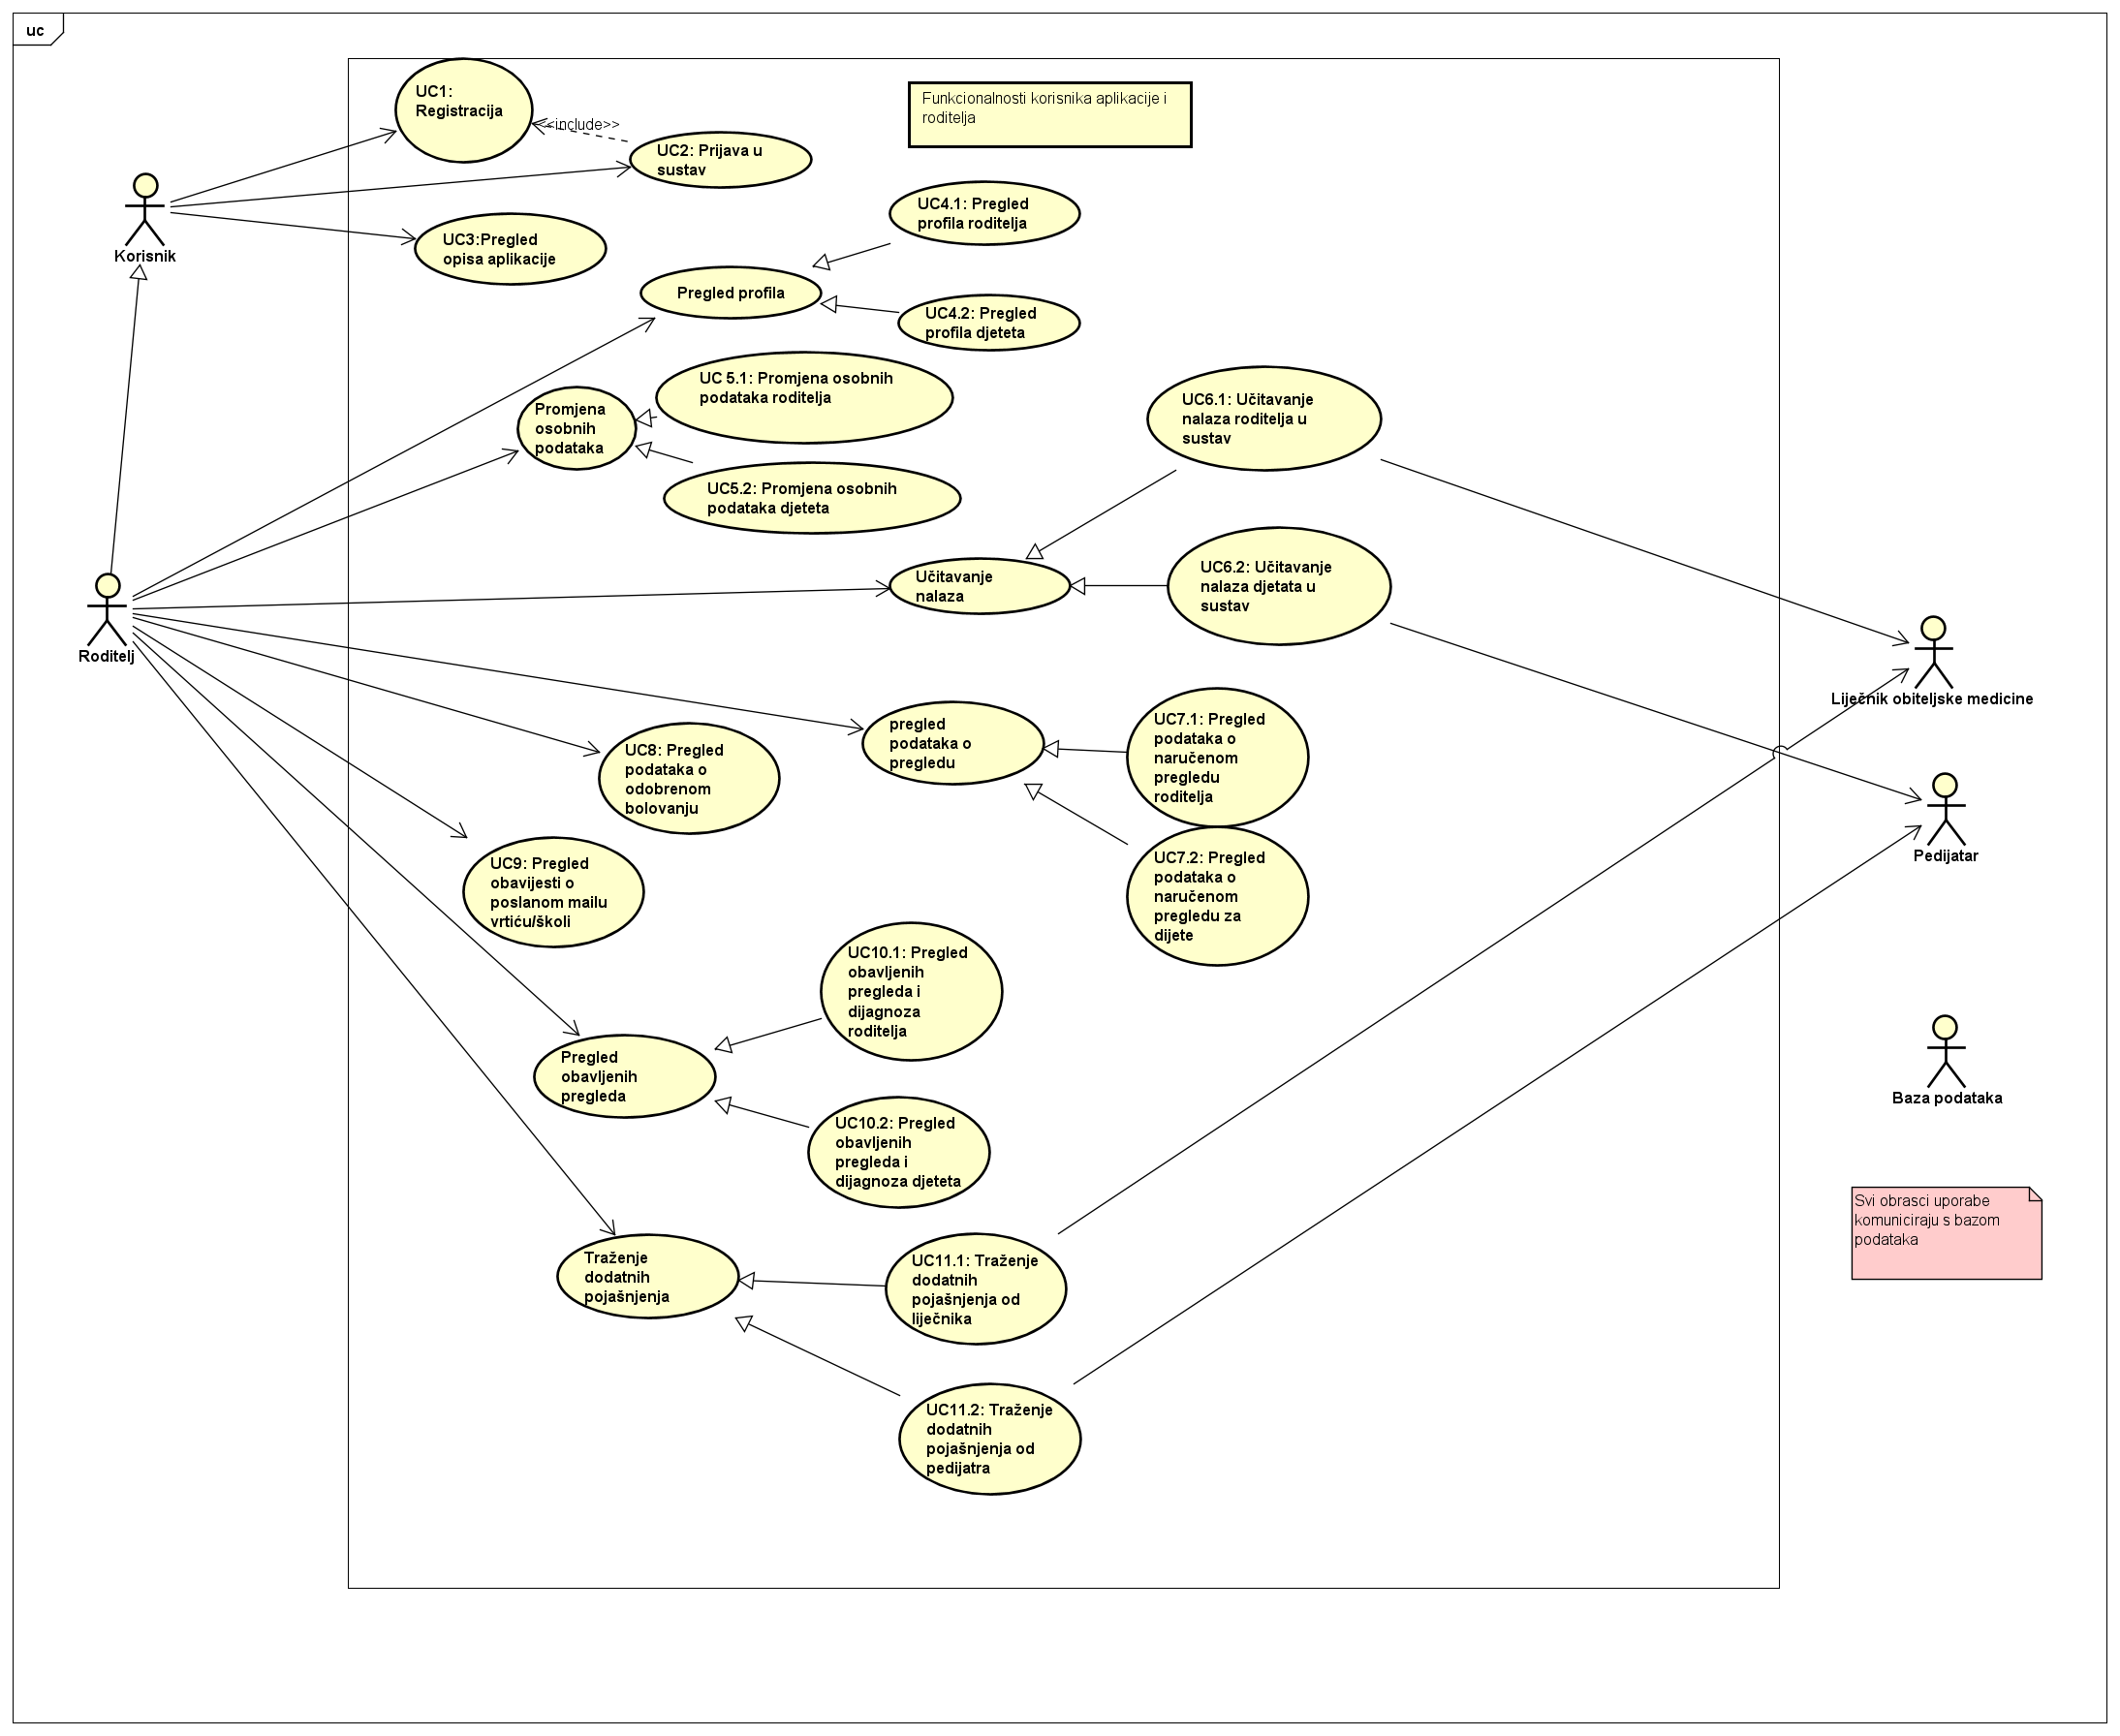
\includegraphics[width=\textwidth]{slike/UCroditelj.PNG} %veličina u odnosu na širinu linije
						\caption{UML dijagram koji opisuje obrasce uporabe korisnika i roditelja}
						\label{fig:promjene3} %label mora biti drugaciji za svaku sliku
					\end{figure}
					
					Referenciranje slike \ref{fig:promjene3} u tekstu.
					
					\begin{figure}[H]
						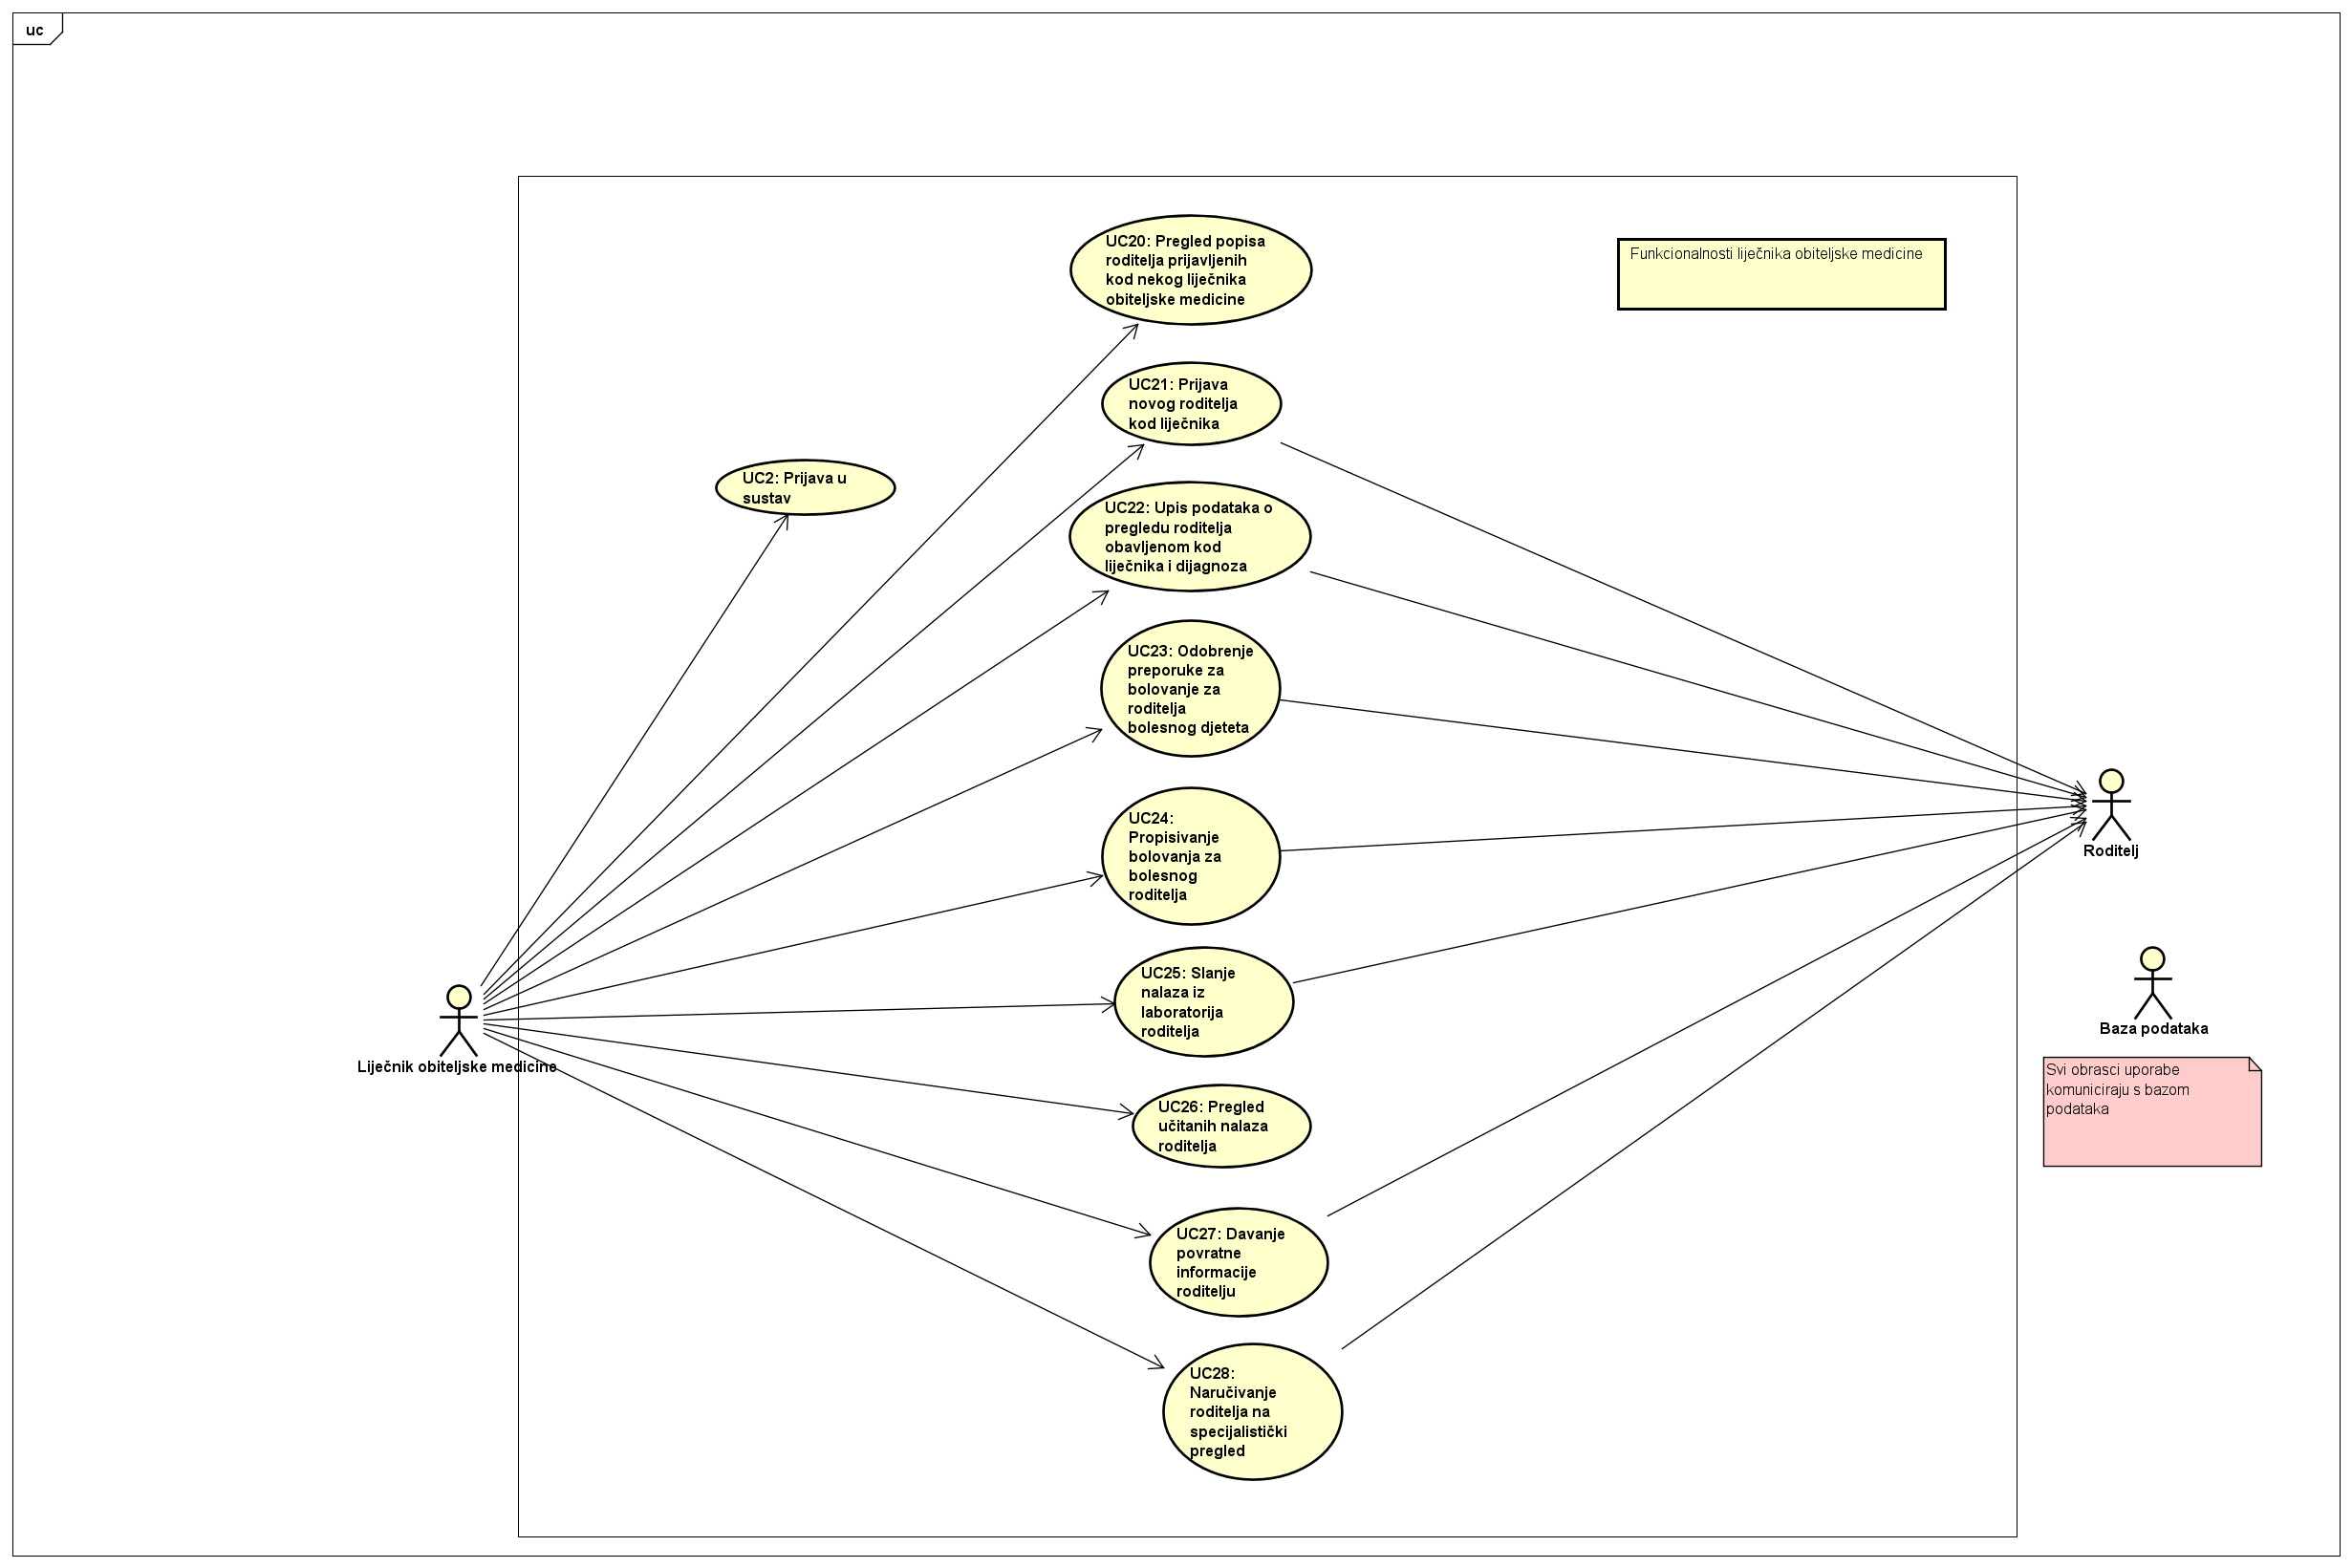
\includegraphics[width=\textwidth]{slike/UCliječnik.PNG} %veličina u odnosu na širinu linije
						\caption{UML dijagram koji opisuje obrasce uporabe liječnika}
						\label{fig:promjene4} %label mora biti drugaciji za svaku sliku
					\end{figure}
					
					Referenciranje slike \ref{fig:promjene4} u tekstu.
					
					\begin{figure}[H]
						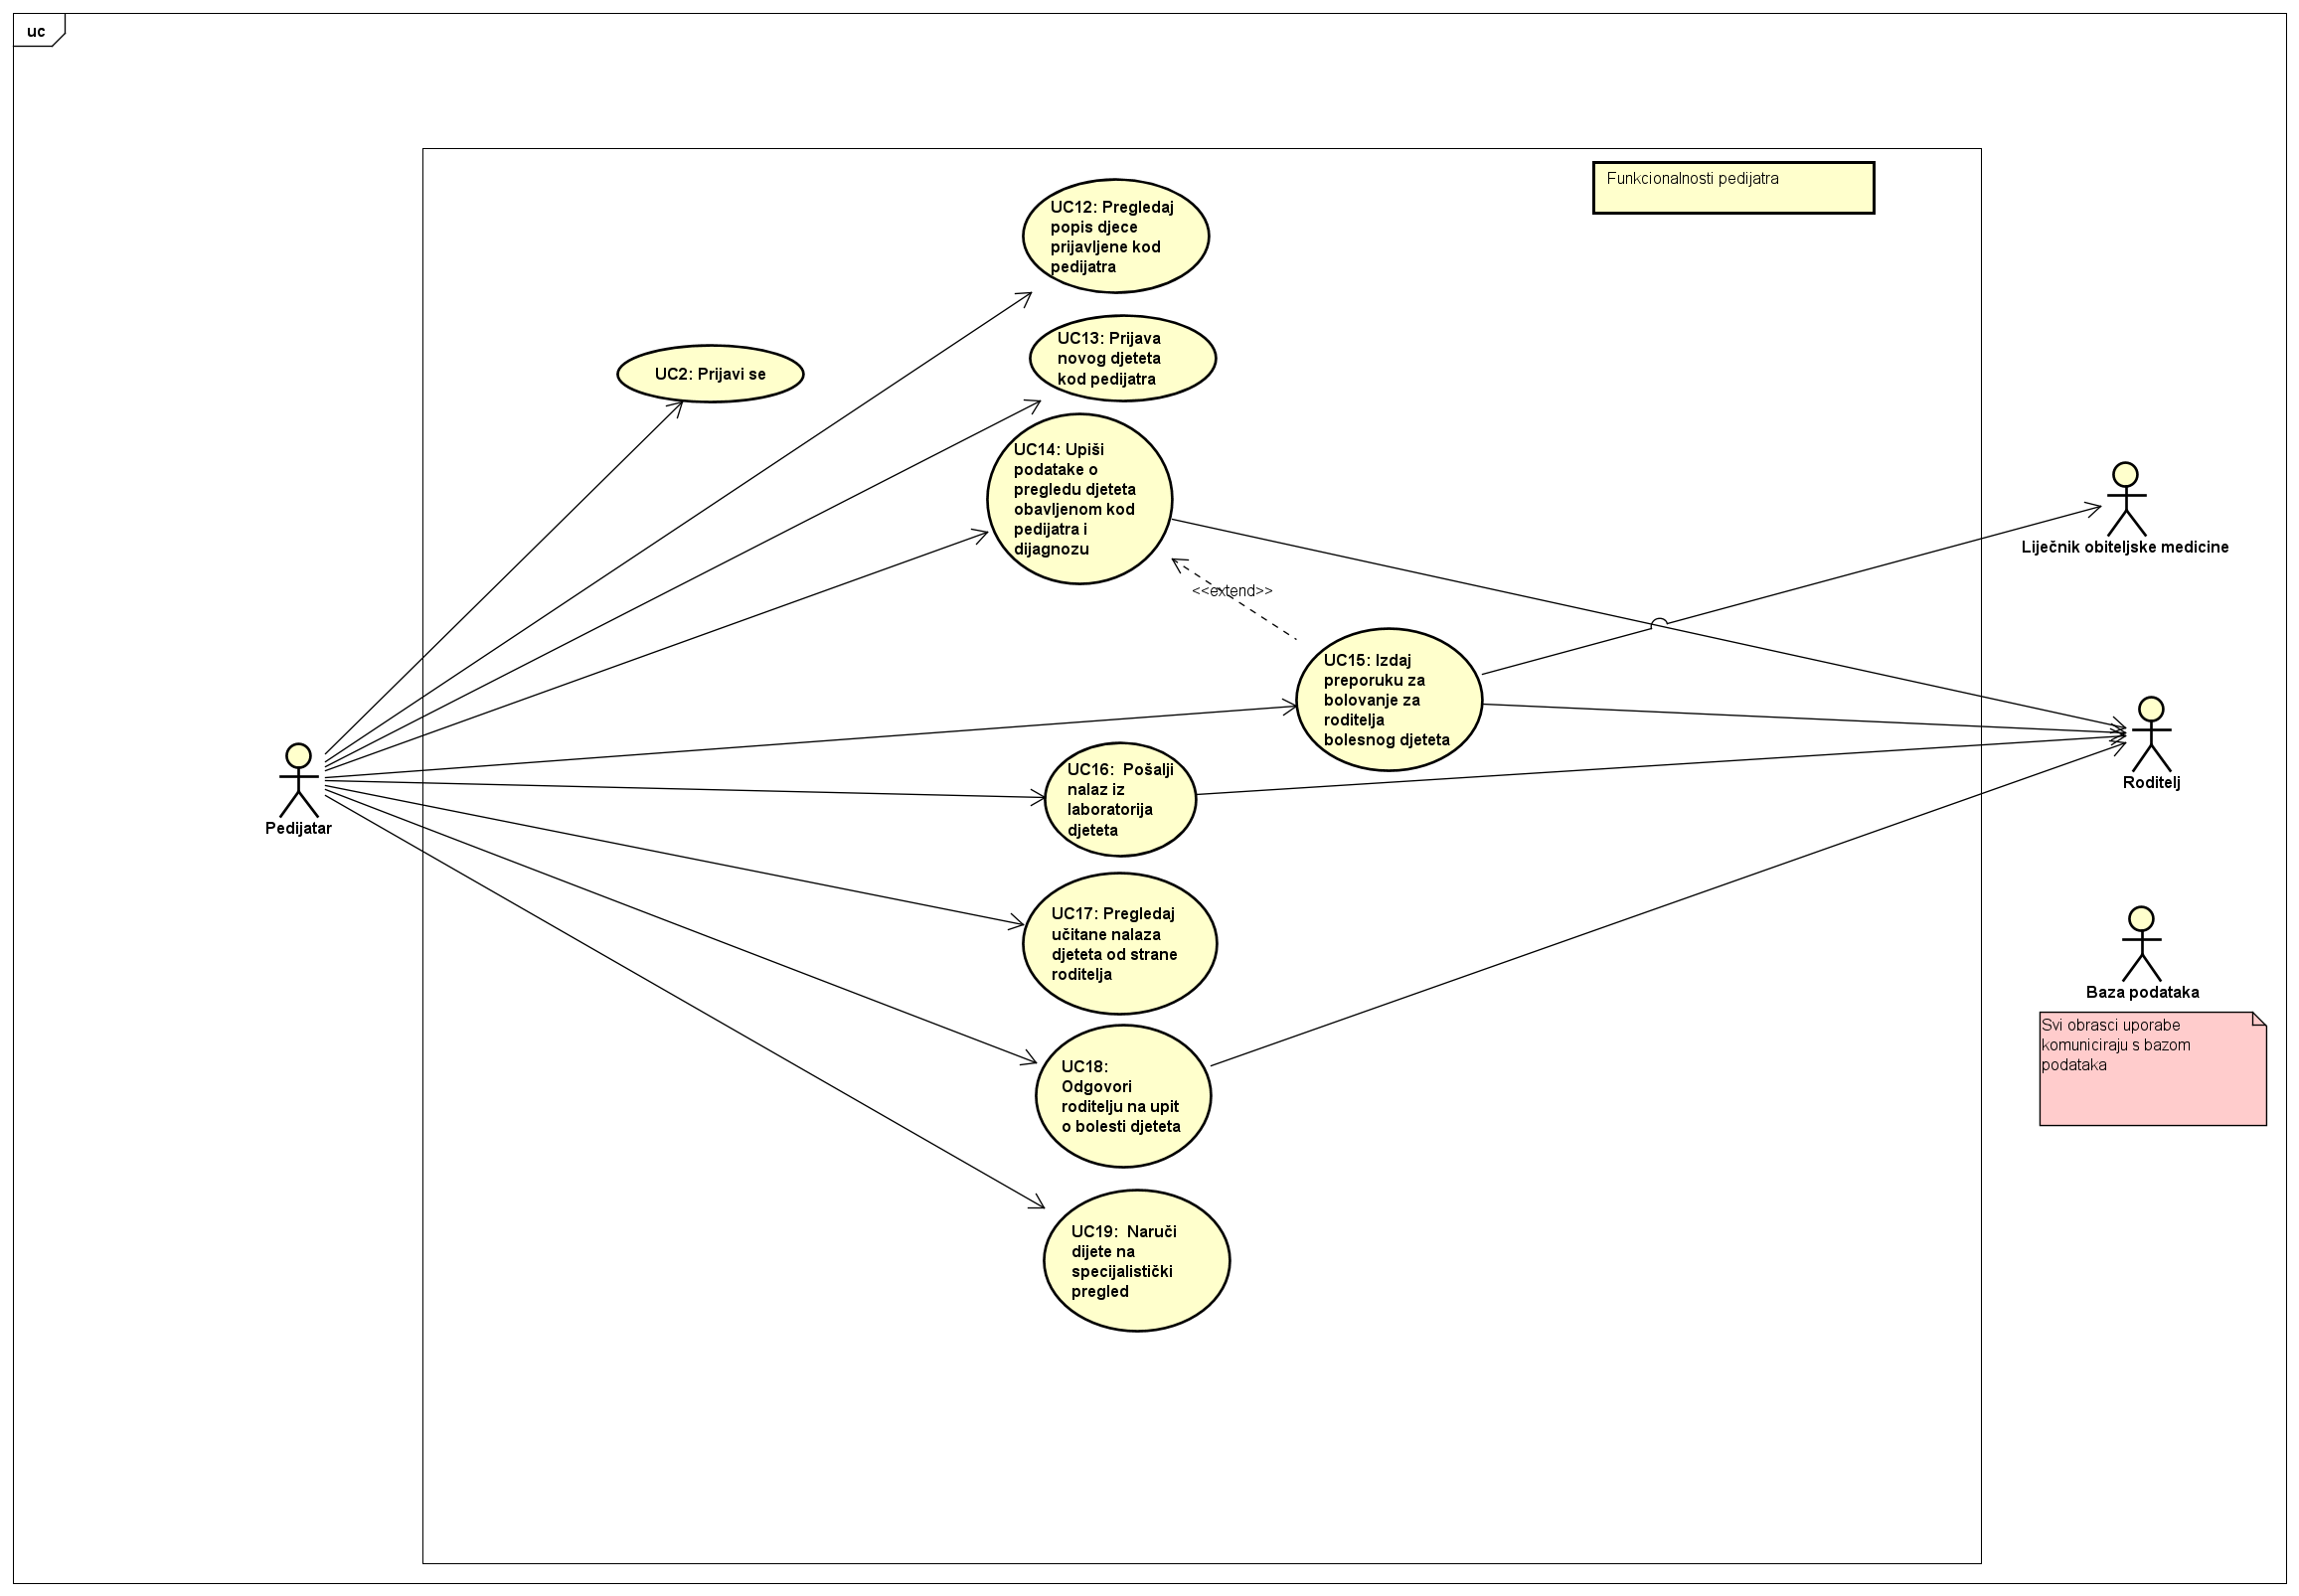
\includegraphics[width=\textwidth]{slike/UCpedijatar.PNG} %veličina u odnosu na širinu linije
						\caption{UML dijagram koji opisuje obrasce uporabe pedijatra}
						\label{fig:promjene5} %label mora biti drugaciji za svaku sliku
					\end{figure}
					
					Referenciranje slike \ref{fig:promjene5} u tekstu.
					
					\begin{figure}[H]
						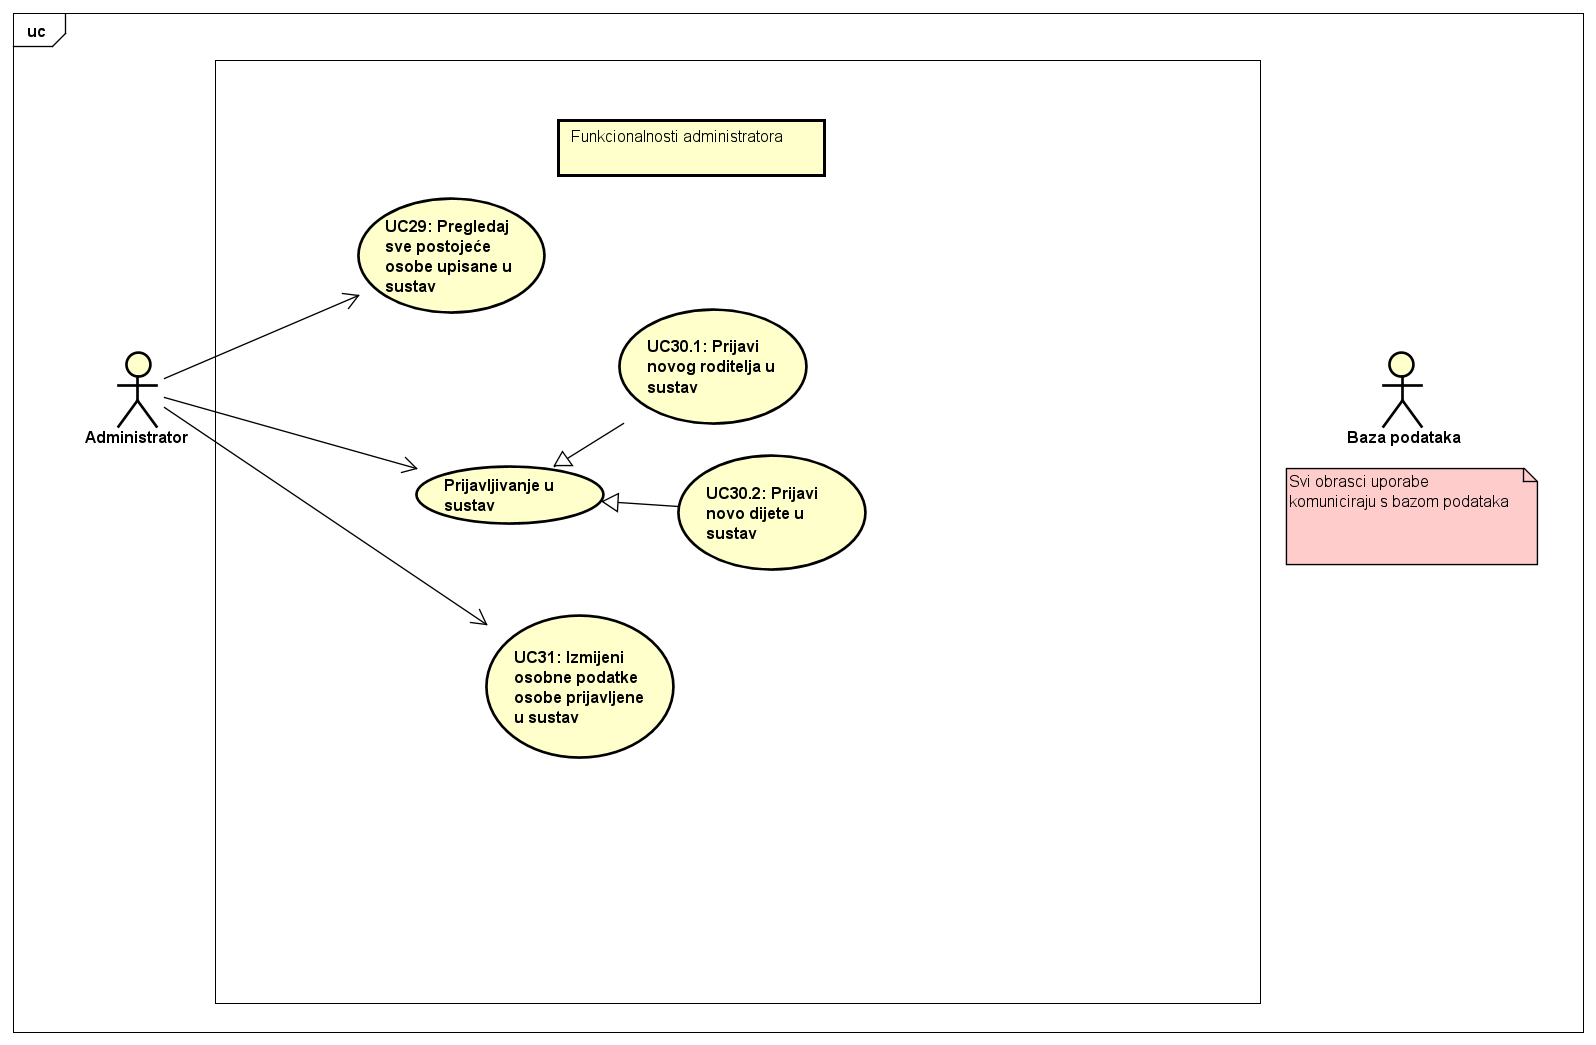
\includegraphics[width=\textwidth]{slike/UCadmin.PNG} %veličina u odnosu na širinu linije
						\caption{UML dijagram koji opisuje obrasce uporabe administratora}
						\label{fig:promjene6} %label mora biti drugaciji za svaku sliku
					\end{figure}
					
					Referenciranje slike \ref{fig:promjene6} u tekstu.
					
				
			\subsection{Sekvencijski dijagrami}
				
				\textbf{\textit{dio 1. revizije}}\\
				
					\textbf{Obrazac uporabe UC6.2 - Učitavanje nalaza djeteta u sustav, UC14 - Upis podataka o pregledu djeteta obavljenom kod pedijatra i dijagnoza, UC15 - Izdavanje preporuke za bolovanje za roditelja bolesnog djeteta, UC16 - Slanje nalaza iz laboratorija djeteta, Pregled učitanih nalaza djeteta od strane roditelja, UC23 - Odobrenje preporuke za bolovanje za roditelja bolesnog djeteta}\\
				
				
				Ulogirani roditelj učitava simptome svog bolesnog djeteta u web aplikaciju koja ga prosljeđuje pedijatru koji dijete naručuje na pregled te nakon pregleda roditelju šalje laboratorijski nalaz te po mogućnosti šalje ispričnicu za školu/vrtić roditelju te preporuku za bolovanje liječniku. Ako liječnik odobri bolovanje roditelju, preko aplikacije mu pošalje potvrdu.
				
				\begin{figure}[H]
					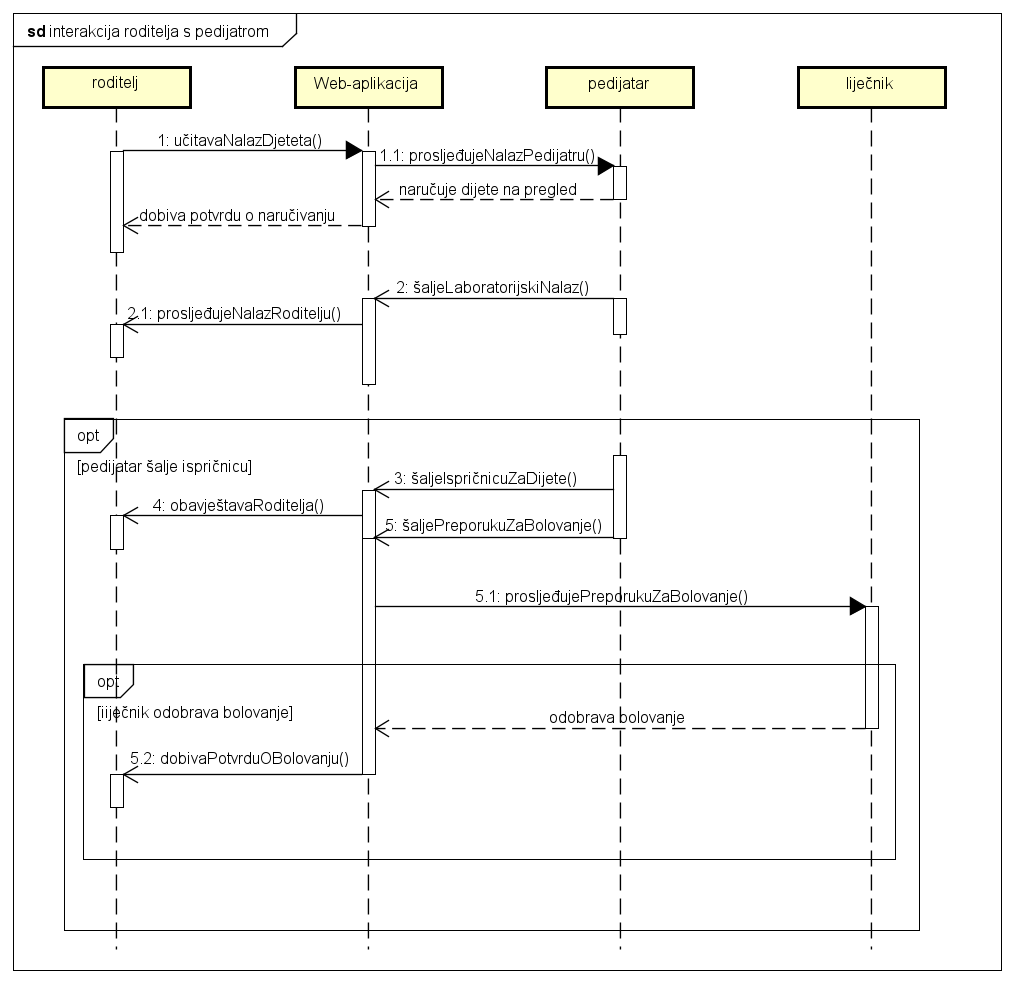
\includegraphics[width=\textwidth]{slike/SDrplW.PNG} %veličina u odnosu na širinu linije
					\caption{Sekvencijski dijagram koji opisuje osnovnu mehaniku naručivanja djeteta i roditelja na pregled}
					\label{fig:promjene7} %label mora biti drugaciji za svaku sliku
				\end{figure}
				
				
				\textbf{Obrazac uporabe UC30.1 - Prijavljivanje novog roditelja u sustav, UC30.2 - Prijavljivanje novog djeteta u sustav}\\
				
				Administrator se ulogirava u sustav i na početnoj stranici bira opciju dodaj roditelja te upisuje njegovo ime, prezime, OIB i datum rođenja. Pritiskom na opciju dodaj u bazu podataka se taj roditelj dodaje. Potom Administrator pokuša upisati novo dijete upisom njegovog imena, prezimena OIB-a, datuma rođenja djeteta te iz liste koja mu se aplikaciji proslijedi iz baze podataka odabere OIB roditelja djeteta kojeg želi upisati u sustav. Potom odabere opciju Dodaj te se baza podataka obnovi.
				\eject
				
				\begin{figure}[H]
					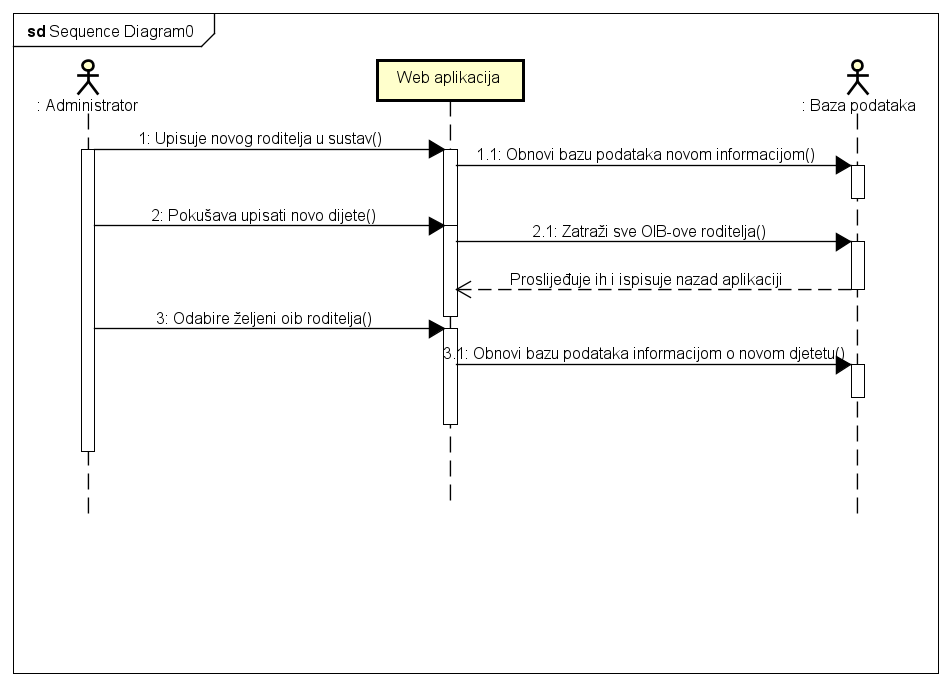
\includegraphics[width=\textwidth]{slike/SDadminapp.PNG} %veličina u odnosu na širinu linije
					\caption{Sekvencijski dijagram za UC30.1 i UC30.2}
					\label{fig:promjene8} %label mora biti drugaciji za svaku sliku
				\end{figure}
				
				
				
				\textbf{Obrazac uporabe UC5.1 - Promjena osobnih podataka roditelja, UC5.2 - Promjena osobnih podataka djeteta}\\
			
				
				Klijent se ulogirava u sustav unosom OIB-a i korisničke lozinke. Nakon provjere postoji li korisnički profil s danim podatcima u bazi, popis dostupnih profila se dohvaća iz baze i ispisuje korisniku. Korisnik odabire profil (vlastiti ili djetetov) te poslužitelj dohvaća podatke iz baze i ispisuje korisnički profil. Odabirom opcije "Pregled osobnih podataka" poslužitelj će iz baze dohvatiti osobne podatke korisnika te ih ispisati na ekran. Korisnik potom uređuje podatke te odabirom opcije "spremi" promjene pohranjuje u bazu. Preglednik će zatim dohvatiti početnu stranicu profila i prikazati ju korisniku.
				\eject
				
				\begin{figure}[H]
					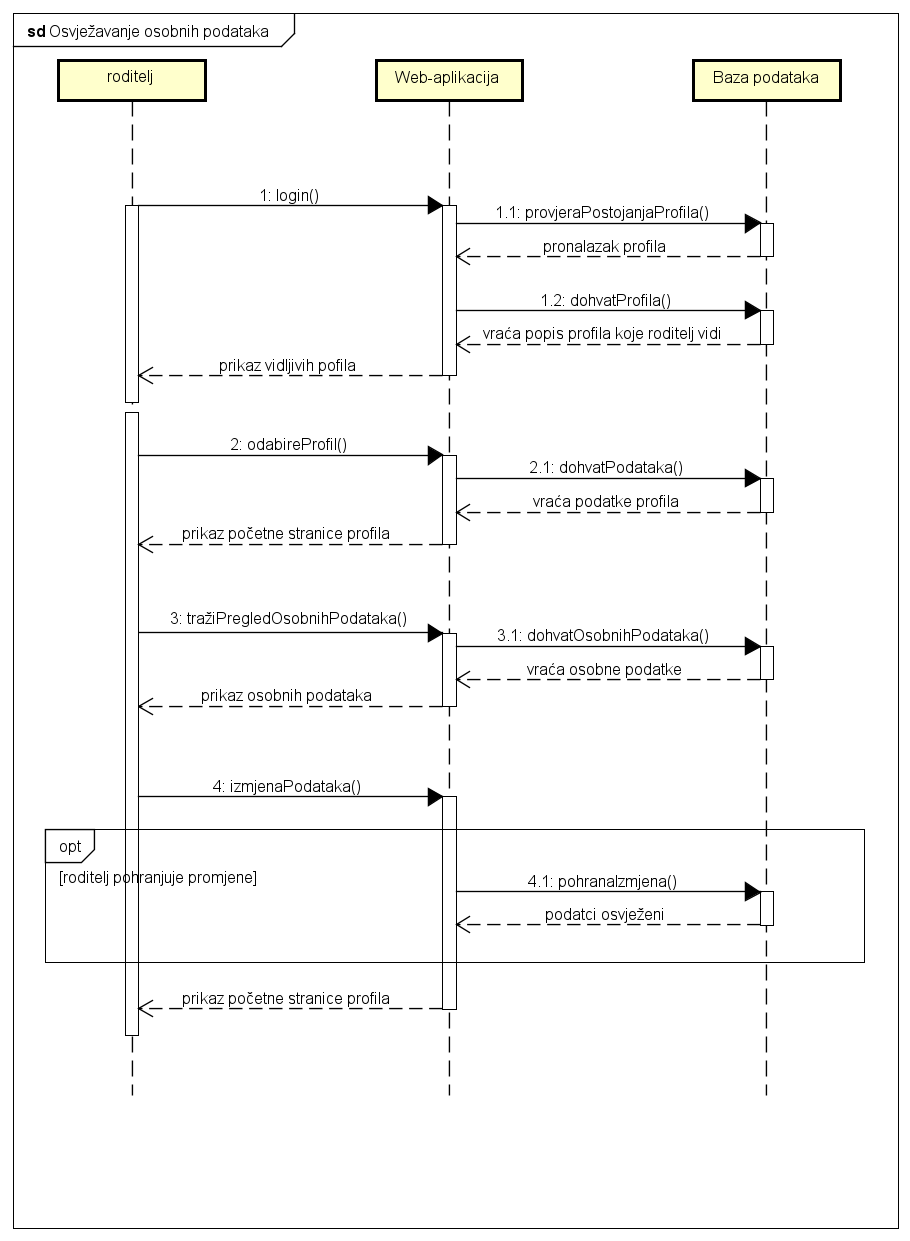
\includegraphics[scale=0.6]{dijagrami/OsobniPodatci.PNG} %veličina slike u odnosu na originalnu datoteku i pozicija slike
					\centering
					\caption{Sekvencijski dijagram za UC5.1 i UC5.2}
					\label{fig:sekvencijski1}
				\end{figure}
				
				\eject
				
				
				
					\textbf{Obrazac uporabe UC13 - Prijava novog djeteta kod pedijatra, UC21 - Prijava novog roditelja kod liječnika}\\
				
				
				Liječnik (pedijatar) se ulogirava u sustav unosom OIB-a i korisničke lozinke. Preglednik poziva bazu i provjerava postoji li korisnički profil u bazi nakon čega iz baze dohvaća upisane pacijente dotičnog korisnika te ih ispisuje na ekran. Korisnik odabire opciju "Prijavi novo(g) dijete/roditelja". Preglednik iz baze dohvaća popis neupisanih pacijenata te ih ispisuje na ekran. Odabirom pacijenta preglednik u bazu upisuje novog pacijenta liječniku/pedijatru, dohvaća osvježenu tablicu upisanih pacijenata te korisniku ispisuje početnu stranicu s upisanim pacijentima.
				
				
				\begin{figure}[H]
					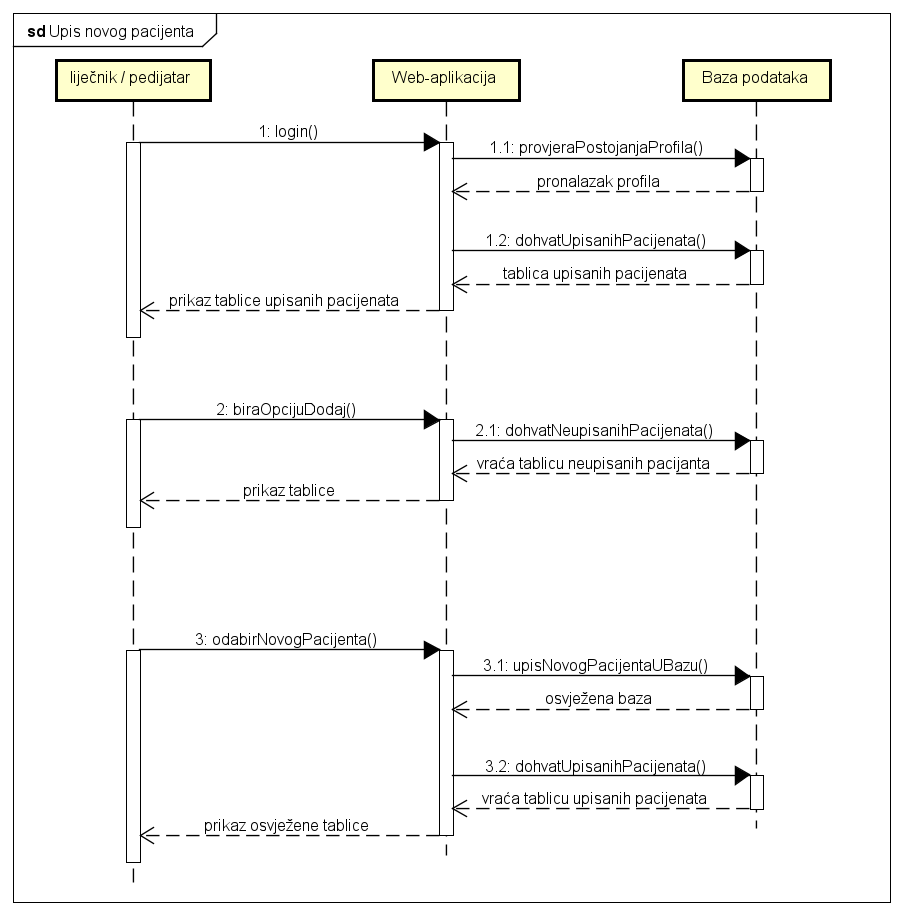
\includegraphics[scale=0.6]{dijagrami/UpisNovogPacijenta.PNG} %veličina slike u odnosu na originalnu datoteku i pozicija slike
					\centering
					\caption{Sekvencijski dijagram za UC13 i UC21}
					\label{fig:sekvencijski2}
				\end{figure}
				
				\eject
	
		\section{Ostali zahtjevi}
		
			\textbf{\textit{dio 1. revizije}}\\
		 
			 \textit{Nefunkcionalni zahtjevi i zahtjevi domene primjene dopunjuju funkcionalne zahtjeve. Oni opisuju \textbf{kako se sustav treba ponašati} i koja \textbf{ograničenja} treba poštivati (performanse, korisničko iskustvo, pouzdanost, standardi kvalitete, sigurnost...). Primjeri takvih zahtjeva u Vašem projektu mogu biti: podržani jezici korisničkog sučelja, vrijeme odziva, najveći mogući podržani broj korisnika, podržane web/mobilne platforme, razina zaštite (protokoli komunikacije, kriptiranje...)... Svaki takav zahtjev potrebno je navesti u jednoj ili dvije rečenice.}
			 
			 
			 
	